\documentclass[letterpaper]{article}
\usepackage[margin=0in]{geometry}
\pdfmapfile{+cm.map}
\usepackage{type1cm}
\usepackage{tikz}
\pagestyle{empty}
\setlength{\parindent}{0pt}
\hyphenpenalty=10000
\exhyphenpenalty=10000
\begin{document}
\begin{tikzpicture}[remember picture,overlay,x=1in,y=-1in]
\begin{scope}[shift={(current page.north west)}]
\node[anchor=north west,inner sep=0pt,text width=7.4in,align=left,font=\sffamily\fontsize{10.8}{13.50}\selectfont] at (0.55,0.36) {\bfseries Week 14 / Polygon triangulations and flips / Grades 2--3};
\node[anchor=north west,inner sep=0pt,text width=7.2in,align=left,font=\sffamily\fontsize{12.3}{15.38}\selectfont] at (0.65,0.91) {Fill the whole polygon with triangles, using straight lines between printed corners. Lines inside a polygon may meet at corners but may not cross. Keep the corner labels fixed, even if you turn the page. Use tracing paper to change printed lines.};
\node[anchor=north west,inner sep=0pt,text width=7.2in,align=left,font=\sffamily\fontsize{13.4}{16.75}\selectfont] at (0.65,1.78) {\textbf{Problem 1:} Fill each polygon in two different ways. Can the two fillings of one polygon have different numbers of triangles?};
\begin{scope}
% polygon: regular n=6
\coordinate (v0) at (3.0000,2.6000);
\coordinate (v1) at (4.5155,3.4750);
\coordinate (v2) at (4.5155,5.2250);
\coordinate (v3) at (3.0000,6.1000);
\coordinate (v4) at (1.4845,5.2250);
\coordinate (v5) at (1.4845,3.4750);
\draw[line width=0.95pt,line join=round] (v0) -- (v1) -- (v2) -- (v3) -- (v4) -- (v5) -- cycle;
\fill (v0) circle[radius=0.022in];
\node[inner sep=0pt,font=\sffamily\fontsize{13}{14}\selectfont] at (3.0000,2.4100) {A};
\fill (v1) circle[radius=0.022in];
\node[inner sep=0pt,font=\sffamily\fontsize{13}{14}\selectfont] at (4.6801,3.3800) {B};
\fill (v2) circle[radius=0.022in];
\node[inner sep=0pt,font=\sffamily\fontsize{13}{14}\selectfont] at (4.6801,5.3200) {C};
\fill (v3) circle[radius=0.022in];
\node[inner sep=0pt,font=\sffamily\fontsize{13}{14}\selectfont] at (3.0000,6.2900) {D};
\fill (v4) circle[radius=0.022in];
\node[inner sep=0pt,font=\sffamily\fontsize{13}{14}\selectfont] at (1.3199,5.3200) {E};
\fill (v5) circle[radius=0.022in];
\node[inner sep=0pt,font=\sffamily\fontsize{13}{14}\selectfont] at (1.3199,3.3800) {F};
\end{scope}
\begin{scope}
% polygon: regular n=6
\coordinate (v0) at (6.7000,2.7050);
\coordinate (v1) at (7.2846,3.0425);
\coordinate (v2) at (7.2846,3.7175);
\coordinate (v3) at (6.7000,4.0550);
\coordinate (v4) at (6.1154,3.7175);
\coordinate (v5) at (6.1154,3.0425);
\draw[line width=0.95pt,line join=round] (v0) -- (v1) -- (v2) -- (v3) -- (v4) -- (v5) -- cycle;
\fill (v0) circle[radius=0.014in];
\node[inner sep=0pt,font=\sffamily\fontsize{8}{14}\selectfont] at (6.7000,2.5850) {A};
\fill (v1) circle[radius=0.014in];
\node[inner sep=0pt,font=\sffamily\fontsize{8}{14}\selectfont] at (7.3885,2.9825) {B};
\fill (v2) circle[radius=0.014in];
\node[inner sep=0pt,font=\sffamily\fontsize{8}{14}\selectfont] at (7.3885,3.7775) {C};
\fill (v3) circle[radius=0.014in];
\node[inner sep=0pt,font=\sffamily\fontsize{8}{14}\selectfont] at (6.7000,4.1750) {D};
\fill (v4) circle[radius=0.014in];
\node[inner sep=0pt,font=\sffamily\fontsize{8}{14}\selectfont] at (6.0115,3.7775) {E};
\fill (v5) circle[radius=0.014in];
\node[inner sep=0pt,font=\sffamily\fontsize{8}{14}\selectfont] at (6.0115,2.9825) {F};
\end{scope}
\begin{scope}
% polygon: regular n=6
\coordinate (v0) at (6.7000,4.6450);
\coordinate (v1) at (7.2846,4.9825);
\coordinate (v2) at (7.2846,5.6575);
\coordinate (v3) at (6.7000,5.9950);
\coordinate (v4) at (6.1154,5.6575);
\coordinate (v5) at (6.1154,4.9825);
\draw[line width=0.95pt,line join=round] (v0) -- (v1) -- (v2) -- (v3) -- (v4) -- (v5) -- cycle;
\fill (v0) circle[radius=0.014in];
\node[inner sep=0pt,font=\sffamily\fontsize{8}{14}\selectfont] at (6.7000,4.5250) {A};
\fill (v1) circle[radius=0.014in];
\node[inner sep=0pt,font=\sffamily\fontsize{8}{14}\selectfont] at (7.3885,4.9225) {B};
\fill (v2) circle[radius=0.014in];
\node[inner sep=0pt,font=\sffamily\fontsize{8}{14}\selectfont] at (7.3885,5.7175) {C};
\fill (v3) circle[radius=0.014in];
\node[inner sep=0pt,font=\sffamily\fontsize{8}{14}\selectfont] at (6.7000,6.1150) {D};
\fill (v4) circle[radius=0.014in];
\node[inner sep=0pt,font=\sffamily\fontsize{8}{14}\selectfont] at (6.0115,5.7175) {E};
\fill (v5) circle[radius=0.014in];
\node[inner sep=0pt,font=\sffamily\fontsize{8}{14}\selectfont] at (6.0115,4.9225) {F};
\end{scope}
\begin{scope}
% polygon: regular n=7
\coordinate (v0) at (3.0000,6.8500);
\coordinate (v1) at (4.1516,7.4046);
\coordinate (v2) at (4.4360,8.6507);
\coordinate (v3) at (3.6391,9.6500);
\coordinate (v4) at (2.3609,9.6500);
\coordinate (v5) at (1.5640,8.6507);
\coordinate (v6) at (1.8484,7.4046);
\draw[line width=0.95pt,line join=round] (v0) -- (v1) -- (v2) -- (v3) -- (v4) -- (v5) -- (v6) -- cycle;
\fill (v0) circle[radius=0.022in];
\node[inner sep=0pt,font=\sffamily\fontsize{13}{14}\selectfont] at (3.0000,6.6600) {A};
\fill (v1) circle[radius=0.022in];
\node[inner sep=0pt,font=\sffamily\fontsize{13}{14}\selectfont] at (4.3047,7.2921) {B};
\fill (v2) circle[radius=0.022in];
\node[inner sep=0pt,font=\sffamily\fontsize{13}{14}\selectfont] at (4.6190,8.7018) {C};
\fill (v3) circle[radius=0.022in];
\node[inner sep=0pt,font=\sffamily\fontsize{13}{14}\selectfont] at (3.7180,9.8228) {D};
\fill (v4) circle[radius=0.022in];
\node[inner sep=0pt,font=\sffamily\fontsize{13}{14}\selectfont] at (2.2820,9.8228) {E};
\fill (v5) circle[radius=0.022in];
\node[inner sep=0pt,font=\sffamily\fontsize{13}{14}\selectfont] at (1.3810,8.7018) {F};
\fill (v6) circle[radius=0.022in];
\node[inner sep=0pt,font=\sffamily\fontsize{13}{14}\selectfont] at (1.6953,7.2921) {G};
\end{scope}
\begin{scope}
% polygon: regular n=7
\coordinate (v0) at (6.7000,6.9250);
\coordinate (v1) at (7.1318,7.1330);
\coordinate (v2) at (7.2385,7.6003);
\coordinate (v3) at (6.9397,7.9750);
\coordinate (v4) at (6.4603,7.9750);
\coordinate (v5) at (6.1615,7.6003);
\coordinate (v6) at (6.2682,7.1330);
\draw[line width=0.95pt,line join=round] (v0) -- (v1) -- (v2) -- (v3) -- (v4) -- (v5) -- (v6) -- cycle;
\fill (v0) circle[radius=0.014in];
\node[inner sep=0pt,font=\sffamily\fontsize{8}{14}\selectfont] at (6.7000,6.8050) {A};
\fill (v1) circle[radius=0.014in];
\node[inner sep=0pt,font=\sffamily\fontsize{8}{14}\selectfont] at (7.2286,7.0620) {B};
\fill (v2) circle[radius=0.014in];
\node[inner sep=0pt,font=\sffamily\fontsize{8}{14}\selectfont] at (7.3541,7.6325) {C};
\fill (v3) circle[radius=0.014in];
\node[inner sep=0pt,font=\sffamily\fontsize{8}{14}\selectfont] at (6.9895,8.0842) {D};
\fill (v4) circle[radius=0.014in];
\node[inner sep=0pt,font=\sffamily\fontsize{8}{14}\selectfont] at (6.4105,8.0842) {E};
\fill (v5) circle[radius=0.014in];
\node[inner sep=0pt,font=\sffamily\fontsize{8}{14}\selectfont] at (6.0459,7.6325) {F};
\fill (v6) circle[radius=0.014in];
\node[inner sep=0pt,font=\sffamily\fontsize{8}{14}\selectfont] at (6.1714,7.0620) {G};
\end{scope}
\begin{scope}
% polygon: regular n=7
\coordinate (v0) at (6.7000,8.5250);
\coordinate (v1) at (7.1318,8.7330);
\coordinate (v2) at (7.2385,9.2003);
\coordinate (v3) at (6.9397,9.5750);
\coordinate (v4) at (6.4603,9.5750);
\coordinate (v5) at (6.1615,9.2003);
\coordinate (v6) at (6.2682,8.7330);
\draw[line width=0.95pt,line join=round] (v0) -- (v1) -- (v2) -- (v3) -- (v4) -- (v5) -- (v6) -- cycle;
\fill (v0) circle[radius=0.014in];
\node[inner sep=0pt,font=\sffamily\fontsize{8}{14}\selectfont] at (6.7000,8.4050) {A};
\fill (v1) circle[radius=0.014in];
\node[inner sep=0pt,font=\sffamily\fontsize{8}{14}\selectfont] at (7.2286,8.6620) {B};
\fill (v2) circle[radius=0.014in];
\node[inner sep=0pt,font=\sffamily\fontsize{8}{14}\selectfont] at (7.3541,9.2325) {C};
\fill (v3) circle[radius=0.014in];
\node[inner sep=0pt,font=\sffamily\fontsize{8}{14}\selectfont] at (6.9895,9.6842) {D};
\fill (v4) circle[radius=0.014in];
\node[inner sep=0pt,font=\sffamily\fontsize{8}{14}\selectfont] at (6.4105,9.6842) {E};
\fill (v5) circle[radius=0.014in];
\node[inner sep=0pt,font=\sffamily\fontsize{8}{14}\selectfont] at (6.0459,9.2325) {F};
\fill (v6) circle[radius=0.014in];
\node[inner sep=0pt,font=\sffamily\fontsize{8}{14}\selectfont] at (6.1714,8.6620) {G};
\end{scope}
\node[anchor=north west,inner sep=0pt,text width=6.9in,align=left,font=\sffamily\fontsize{9}{11.25}\selectfont] at (0.55,10.48) {Bellingham Math Circle / Week 14 / F14-23-v2};
\node[anchor=north west,inner sep=0pt,text width=0.36in,align=left,font=\sffamily\fontsize{9}{11.25}\selectfont] at (7.56,10.48) {1};
\end{scope}
\end{tikzpicture}
\null
\newpage
\begin{tikzpicture}[remember picture,overlay,x=1in,y=-1in]
\begin{scope}[shift={(current page.north west)}]
\node[anchor=north west,inner sep=0pt,text width=7.4in,align=left,font=\sffamily\fontsize{10.8}{13.50}\selectfont] at (0.55,0.36) {\bfseries Week 14 / Polygon triangulations and flips / Grades 2--3};
\node[anchor=north west,inner sep=0pt,text width=7.2in,align=left,font=\sffamily\fontsize{13.4}{16.75}\selectfont] at (0.65,0.91) {\textbf{Problem 2:} Find every filling of this five-corner polygon. Organize your drawings so that you can explain why none are missing.};
\begin{scope}
% polygon: regular n=5
\coordinate (v0) at (4.2500,2.5750);
\coordinate (v1) at (6.0112,3.8546);
\coordinate (v2) at (5.3385,5.9250);
\coordinate (v3) at (3.1615,5.9250);
\coordinate (v4) at (2.4888,3.8546);
\draw[line width=0.95pt,line join=round] (v0) -- (v1) -- (v2) -- (v3) -- (v4) -- cycle;
\fill (v0) circle[radius=0.022in];
\node[inner sep=0pt,font=\sffamily\fontsize{13}{14}\selectfont] at (4.2500,2.3850) {A};
\fill (v1) circle[radius=0.022in];
\node[inner sep=0pt,font=\sffamily\fontsize{13}{14}\selectfont] at (6.1966,3.8130) {B};
\fill (v2) circle[radius=0.022in];
\node[inner sep=0pt,font=\sffamily\fontsize{13}{14}\selectfont] at (5.4420,6.0843) {C};
\fill (v3) circle[radius=0.022in];
\node[inner sep=0pt,font=\sffamily\fontsize{13}{14}\selectfont] at (3.0580,6.0843) {D};
\fill (v4) circle[radius=0.022in];
\node[inner sep=0pt,font=\sffamily\fontsize{13}{14}\selectfont] at (2.3034,3.8130) {E};
\end{scope}
\begin{scope}
% polygon: regular n=5
\coordinate (v0) at (1.3500,6.9900);
\coordinate (v1) at (1.8337,7.3414);
\coordinate (v2) at (1.6489,7.9100);
\coordinate (v3) at (1.0511,7.9100);
\coordinate (v4) at (0.8663,7.3414);
\draw[line width=0.95pt,line join=round] (v0) -- (v1) -- (v2) -- (v3) -- (v4) -- cycle;
\fill (v0) circle[radius=0.014in];
\node[inner sep=0pt,font=\sffamily\fontsize{8}{14}\selectfont] at (1.3500,6.8700) {A};
\fill (v1) circle[radius=0.014in];
\node[inner sep=0pt,font=\sffamily\fontsize{8}{14}\selectfont] at (1.9508,7.3151) {B};
\fill (v2) circle[radius=0.014in];
\node[inner sep=0pt,font=\sffamily\fontsize{8}{14}\selectfont] at (1.7143,8.0106) {C};
\fill (v3) circle[radius=0.014in];
\node[inner sep=0pt,font=\sffamily\fontsize{8}{14}\selectfont] at (0.9857,8.0106) {D};
\fill (v4) circle[radius=0.014in];
\node[inner sep=0pt,font=\sffamily\fontsize{8}{14}\selectfont] at (0.7492,7.3151) {E};
\end{scope}
\begin{scope}
% polygon: regular n=5
\coordinate (v0) at (3.2800,6.9900);
\coordinate (v1) at (3.7637,7.3414);
\coordinate (v2) at (3.5789,7.9100);
\coordinate (v3) at (2.9811,7.9100);
\coordinate (v4) at (2.7963,7.3414);
\draw[line width=0.95pt,line join=round] (v0) -- (v1) -- (v2) -- (v3) -- (v4) -- cycle;
\fill (v0) circle[radius=0.014in];
\node[inner sep=0pt,font=\sffamily\fontsize{8}{14}\selectfont] at (3.2800,6.8700) {A};
\fill (v1) circle[radius=0.014in];
\node[inner sep=0pt,font=\sffamily\fontsize{8}{14}\selectfont] at (3.8808,7.3151) {B};
\fill (v2) circle[radius=0.014in];
\node[inner sep=0pt,font=\sffamily\fontsize{8}{14}\selectfont] at (3.6443,8.0106) {C};
\fill (v3) circle[radius=0.014in];
\node[inner sep=0pt,font=\sffamily\fontsize{8}{14}\selectfont] at (2.9157,8.0106) {D};
\fill (v4) circle[radius=0.014in];
\node[inner sep=0pt,font=\sffamily\fontsize{8}{14}\selectfont] at (2.6792,7.3151) {E};
\end{scope}
\begin{scope}
% polygon: regular n=5
\coordinate (v0) at (5.2200,6.9900);
\coordinate (v1) at (5.7037,7.3414);
\coordinate (v2) at (5.5189,7.9100);
\coordinate (v3) at (4.9211,7.9100);
\coordinate (v4) at (4.7363,7.3414);
\draw[line width=0.95pt,line join=round] (v0) -- (v1) -- (v2) -- (v3) -- (v4) -- cycle;
\fill (v0) circle[radius=0.014in];
\node[inner sep=0pt,font=\sffamily\fontsize{8}{14}\selectfont] at (5.2200,6.8700) {A};
\fill (v1) circle[radius=0.014in];
\node[inner sep=0pt,font=\sffamily\fontsize{8}{14}\selectfont] at (5.8208,7.3151) {B};
\fill (v2) circle[radius=0.014in];
\node[inner sep=0pt,font=\sffamily\fontsize{8}{14}\selectfont] at (5.5843,8.0106) {C};
\fill (v3) circle[radius=0.014in];
\node[inner sep=0pt,font=\sffamily\fontsize{8}{14}\selectfont] at (4.8557,8.0106) {D};
\fill (v4) circle[radius=0.014in];
\node[inner sep=0pt,font=\sffamily\fontsize{8}{14}\selectfont] at (4.6192,7.3151) {E};
\end{scope}
\begin{scope}
% polygon: regular n=5
\coordinate (v0) at (7.1500,6.9900);
\coordinate (v1) at (7.6337,7.3414);
\coordinate (v2) at (7.4489,7.9100);
\coordinate (v3) at (6.8511,7.9100);
\coordinate (v4) at (6.6663,7.3414);
\draw[line width=0.95pt,line join=round] (v0) -- (v1) -- (v2) -- (v3) -- (v4) -- cycle;
\fill (v0) circle[radius=0.014in];
\node[inner sep=0pt,font=\sffamily\fontsize{8}{14}\selectfont] at (7.1500,6.8700) {A};
\fill (v1) circle[radius=0.014in];
\node[inner sep=0pt,font=\sffamily\fontsize{8}{14}\selectfont] at (7.7508,7.3151) {B};
\fill (v2) circle[radius=0.014in];
\node[inner sep=0pt,font=\sffamily\fontsize{8}{14}\selectfont] at (7.5143,8.0106) {C};
\fill (v3) circle[radius=0.014in];
\node[inner sep=0pt,font=\sffamily\fontsize{8}{14}\selectfont] at (6.7857,8.0106) {D};
\fill (v4) circle[radius=0.014in];
\node[inner sep=0pt,font=\sffamily\fontsize{8}{14}\selectfont] at (6.5492,7.3151) {E};
\end{scope}
\begin{scope}
% polygon: regular n=5
\coordinate (v0) at (1.3500,8.4900);
\coordinate (v1) at (1.8337,8.8414);
\coordinate (v2) at (1.6489,9.4100);
\coordinate (v3) at (1.0511,9.4100);
\coordinate (v4) at (0.8663,8.8414);
\draw[line width=0.95pt,line join=round] (v0) -- (v1) -- (v2) -- (v3) -- (v4) -- cycle;
\fill (v0) circle[radius=0.014in];
\node[inner sep=0pt,font=\sffamily\fontsize{8}{14}\selectfont] at (1.3500,8.3700) {A};
\fill (v1) circle[radius=0.014in];
\node[inner sep=0pt,font=\sffamily\fontsize{8}{14}\selectfont] at (1.9508,8.8151) {B};
\fill (v2) circle[radius=0.014in];
\node[inner sep=0pt,font=\sffamily\fontsize{8}{14}\selectfont] at (1.7143,9.5106) {C};
\fill (v3) circle[radius=0.014in];
\node[inner sep=0pt,font=\sffamily\fontsize{8}{14}\selectfont] at (0.9857,9.5106) {D};
\fill (v4) circle[radius=0.014in];
\node[inner sep=0pt,font=\sffamily\fontsize{8}{14}\selectfont] at (0.7492,8.8151) {E};
\end{scope}
\begin{scope}
% polygon: regular n=5
\coordinate (v0) at (3.2800,8.4900);
\coordinate (v1) at (3.7637,8.8414);
\coordinate (v2) at (3.5789,9.4100);
\coordinate (v3) at (2.9811,9.4100);
\coordinate (v4) at (2.7963,8.8414);
\draw[line width=0.95pt,line join=round] (v0) -- (v1) -- (v2) -- (v3) -- (v4) -- cycle;
\fill (v0) circle[radius=0.014in];
\node[inner sep=0pt,font=\sffamily\fontsize{8}{14}\selectfont] at (3.2800,8.3700) {A};
\fill (v1) circle[radius=0.014in];
\node[inner sep=0pt,font=\sffamily\fontsize{8}{14}\selectfont] at (3.8808,8.8151) {B};
\fill (v2) circle[radius=0.014in];
\node[inner sep=0pt,font=\sffamily\fontsize{8}{14}\selectfont] at (3.6443,9.5106) {C};
\fill (v3) circle[radius=0.014in];
\node[inner sep=0pt,font=\sffamily\fontsize{8}{14}\selectfont] at (2.9157,9.5106) {D};
\fill (v4) circle[radius=0.014in];
\node[inner sep=0pt,font=\sffamily\fontsize{8}{14}\selectfont] at (2.6792,8.8151) {E};
\end{scope}
\begin{scope}
% polygon: regular n=5
\coordinate (v0) at (5.2200,8.4900);
\coordinate (v1) at (5.7037,8.8414);
\coordinate (v2) at (5.5189,9.4100);
\coordinate (v3) at (4.9211,9.4100);
\coordinate (v4) at (4.7363,8.8414);
\draw[line width=0.95pt,line join=round] (v0) -- (v1) -- (v2) -- (v3) -- (v4) -- cycle;
\fill (v0) circle[radius=0.014in];
\node[inner sep=0pt,font=\sffamily\fontsize{8}{14}\selectfont] at (5.2200,8.3700) {A};
\fill (v1) circle[radius=0.014in];
\node[inner sep=0pt,font=\sffamily\fontsize{8}{14}\selectfont] at (5.8208,8.8151) {B};
\fill (v2) circle[radius=0.014in];
\node[inner sep=0pt,font=\sffamily\fontsize{8}{14}\selectfont] at (5.5843,9.5106) {C};
\fill (v3) circle[radius=0.014in];
\node[inner sep=0pt,font=\sffamily\fontsize{8}{14}\selectfont] at (4.8557,9.5106) {D};
\fill (v4) circle[radius=0.014in];
\node[inner sep=0pt,font=\sffamily\fontsize{8}{14}\selectfont] at (4.6192,8.8151) {E};
\end{scope}
\begin{scope}
% polygon: regular n=5
\coordinate (v0) at (7.1500,8.4900);
\coordinate (v1) at (7.6337,8.8414);
\coordinate (v2) at (7.4489,9.4100);
\coordinate (v3) at (6.8511,9.4100);
\coordinate (v4) at (6.6663,8.8414);
\draw[line width=0.95pt,line join=round] (v0) -- (v1) -- (v2) -- (v3) -- (v4) -- cycle;
\fill (v0) circle[radius=0.014in];
\node[inner sep=0pt,font=\sffamily\fontsize{8}{14}\selectfont] at (7.1500,8.3700) {A};
\fill (v1) circle[radius=0.014in];
\node[inner sep=0pt,font=\sffamily\fontsize{8}{14}\selectfont] at (7.7508,8.8151) {B};
\fill (v2) circle[radius=0.014in];
\node[inner sep=0pt,font=\sffamily\fontsize{8}{14}\selectfont] at (7.5143,9.5106) {C};
\fill (v3) circle[radius=0.014in];
\node[inner sep=0pt,font=\sffamily\fontsize{8}{14}\selectfont] at (6.7857,9.5106) {D};
\fill (v4) circle[radius=0.014in];
\node[inner sep=0pt,font=\sffamily\fontsize{8}{14}\selectfont] at (6.5492,8.8151) {E};
\end{scope}
\node[anchor=north west,inner sep=0pt,text width=6.9in,align=left,font=\sffamily\fontsize{9}{11.25}\selectfont] at (0.55,10.48) {Bellingham Math Circle / Week 14 / F14-23-v2};
\node[anchor=north west,inner sep=0pt,text width=0.36in,align=left,font=\sffamily\fontsize{9}{11.25}\selectfont] at (7.56,10.48) {2};
\end{scope}
\end{tikzpicture}
\null
\newpage
\begin{tikzpicture}[remember picture,overlay,x=1in,y=-1in]
\begin{scope}[shift={(current page.north west)}]
\node[anchor=north west,inner sep=0pt,text width=7.4in,align=left,font=\sffamily\fontsize{10.8}{13.50}\selectfont] at (0.55,0.36) {\bfseries Week 14 / Polygon triangulations and flips / Grades 2--3};
\node[anchor=north west,inner sep=0pt,text width=7.2in,align=left,font=\sffamily\fontsize{13.4}{16.75}\selectfont] at (0.65,0.91) {\textbf{Problem 3:} Erase one inside line and replace it with a different line so the polygon stays filled with triangles. Find every result of one such change from each drawing.};
\begin{scope}
% polygon: regular n=6
\coordinate (v0) at (2.3500,2.0250);
\coordinate (v1) at (3.8439,2.8875);
\coordinate (v2) at (3.8439,4.6125);
\coordinate (v3) at (2.3500,5.4750);
\coordinate (v4) at (0.8561,4.6125);
\coordinate (v5) at (0.8561,2.8875);
\draw[line width=0.95pt,line join=round] (v0) -- (v1) -- (v2) -- (v3) -- (v4) -- (v5) -- cycle;
\draw[line width=0.85pt] (v0) -- (v2);
\draw[line width=0.85pt] (v0) -- (v3);
\draw[line width=0.85pt] (v0) -- (v4);
\fill (v0) circle[radius=0.022in];
\node[inner sep=0pt,font=\sffamily\fontsize{13}{14}\selectfont] at (2.3500,1.8350) {A};
\fill (v1) circle[radius=0.022in];
\node[inner sep=0pt,font=\sffamily\fontsize{13}{14}\selectfont] at (4.0084,2.7925) {B};
\fill (v2) circle[radius=0.022in];
\node[inner sep=0pt,font=\sffamily\fontsize{13}{14}\selectfont] at (4.0084,4.7075) {C};
\fill (v3) circle[radius=0.022in];
\node[inner sep=0pt,font=\sffamily\fontsize{13}{14}\selectfont] at (2.3500,5.6650) {D};
\fill (v4) circle[radius=0.022in];
\node[inner sep=0pt,font=\sffamily\fontsize{13}{14}\selectfont] at (0.6916,4.7075) {E};
\fill (v5) circle[radius=0.022in];
\node[inner sep=0pt,font=\sffamily\fontsize{13}{14}\selectfont] at (0.6916,2.7925) {F};
\end{scope}
\begin{scope}
% polygon: regular n=6
\coordinate (v0) at (5.2500,2.2000);
\coordinate (v1) at (5.8129,2.5250);
\coordinate (v2) at (5.8129,3.1750);
\coordinate (v3) at (5.2500,3.5000);
\coordinate (v4) at (4.6871,3.1750);
\coordinate (v5) at (4.6871,2.5250);
\draw[line width=0.95pt,line join=round] (v0) -- (v1) -- (v2) -- (v3) -- (v4) -- (v5) -- cycle;
\fill (v0) circle[radius=0.014in];
\node[inner sep=0pt,font=\sffamily\fontsize{8}{14}\selectfont] at (5.2500,2.0800) {A};
\fill (v1) circle[radius=0.014in];
\node[inner sep=0pt,font=\sffamily\fontsize{8}{14}\selectfont] at (5.9168,2.4650) {B};
\fill (v2) circle[radius=0.014in];
\node[inner sep=0pt,font=\sffamily\fontsize{8}{14}\selectfont] at (5.9168,3.2350) {C};
\fill (v3) circle[radius=0.014in];
\node[inner sep=0pt,font=\sffamily\fontsize{8}{14}\selectfont] at (5.2500,3.6200) {D};
\fill (v4) circle[radius=0.014in];
\node[inner sep=0pt,font=\sffamily\fontsize{8}{14}\selectfont] at (4.5832,3.2350) {E};
\fill (v5) circle[radius=0.014in];
\node[inner sep=0pt,font=\sffamily\fontsize{8}{14}\selectfont] at (4.5832,2.4650) {F};
\end{scope}
\begin{scope}
% polygon: regular n=6
\coordinate (v0) at (5.2500,4.0000);
\coordinate (v1) at (5.8129,4.3250);
\coordinate (v2) at (5.8129,4.9750);
\coordinate (v3) at (5.2500,5.3000);
\coordinate (v4) at (4.6871,4.9750);
\coordinate (v5) at (4.6871,4.3250);
\draw[line width=0.95pt,line join=round] (v0) -- (v1) -- (v2) -- (v3) -- (v4) -- (v5) -- cycle;
\fill (v0) circle[radius=0.014in];
\node[inner sep=0pt,font=\sffamily\fontsize{8}{14}\selectfont] at (5.2500,3.8800) {A};
\fill (v1) circle[radius=0.014in];
\node[inner sep=0pt,font=\sffamily\fontsize{8}{14}\selectfont] at (5.9168,4.2650) {B};
\fill (v2) circle[radius=0.014in];
\node[inner sep=0pt,font=\sffamily\fontsize{8}{14}\selectfont] at (5.9168,5.0350) {C};
\fill (v3) circle[radius=0.014in];
\node[inner sep=0pt,font=\sffamily\fontsize{8}{14}\selectfont] at (5.2500,5.4200) {D};
\fill (v4) circle[radius=0.014in];
\node[inner sep=0pt,font=\sffamily\fontsize{8}{14}\selectfont] at (4.5832,5.0350) {E};
\fill (v5) circle[radius=0.014in];
\node[inner sep=0pt,font=\sffamily\fontsize{8}{14}\selectfont] at (4.5832,4.2650) {F};
\end{scope}
\begin{scope}
% polygon: regular n=6
\coordinate (v0) at (7.1500,2.2000);
\coordinate (v1) at (7.7129,2.5250);
\coordinate (v2) at (7.7129,3.1750);
\coordinate (v3) at (7.1500,3.5000);
\coordinate (v4) at (6.5871,3.1750);
\coordinate (v5) at (6.5871,2.5250);
\draw[line width=0.95pt,line join=round] (v0) -- (v1) -- (v2) -- (v3) -- (v4) -- (v5) -- cycle;
\fill (v0) circle[radius=0.014in];
\node[inner sep=0pt,font=\sffamily\fontsize{8}{14}\selectfont] at (7.1500,2.0800) {A};
\fill (v1) circle[radius=0.014in];
\node[inner sep=0pt,font=\sffamily\fontsize{8}{14}\selectfont] at (7.8168,2.4650) {B};
\fill (v2) circle[radius=0.014in];
\node[inner sep=0pt,font=\sffamily\fontsize{8}{14}\selectfont] at (7.8168,3.2350) {C};
\fill (v3) circle[radius=0.014in];
\node[inner sep=0pt,font=\sffamily\fontsize{8}{14}\selectfont] at (7.1500,3.6200) {D};
\fill (v4) circle[radius=0.014in];
\node[inner sep=0pt,font=\sffamily\fontsize{8}{14}\selectfont] at (6.4832,3.2350) {E};
\fill (v5) circle[radius=0.014in];
\node[inner sep=0pt,font=\sffamily\fontsize{8}{14}\selectfont] at (6.4832,2.4650) {F};
\end{scope}
\begin{scope}
% polygon: regular n=6
\coordinate (v0) at (7.1500,4.0000);
\coordinate (v1) at (7.7129,4.3250);
\coordinate (v2) at (7.7129,4.9750);
\coordinate (v3) at (7.1500,5.3000);
\coordinate (v4) at (6.5871,4.9750);
\coordinate (v5) at (6.5871,4.3250);
\draw[line width=0.95pt,line join=round] (v0) -- (v1) -- (v2) -- (v3) -- (v4) -- (v5) -- cycle;
\fill (v0) circle[radius=0.014in];
\node[inner sep=0pt,font=\sffamily\fontsize{8}{14}\selectfont] at (7.1500,3.8800) {A};
\fill (v1) circle[radius=0.014in];
\node[inner sep=0pt,font=\sffamily\fontsize{8}{14}\selectfont] at (7.8168,4.2650) {B};
\fill (v2) circle[radius=0.014in];
\node[inner sep=0pt,font=\sffamily\fontsize{8}{14}\selectfont] at (7.8168,5.0350) {C};
\fill (v3) circle[radius=0.014in];
\node[inner sep=0pt,font=\sffamily\fontsize{8}{14}\selectfont] at (7.1500,5.4200) {D};
\fill (v4) circle[radius=0.014in];
\node[inner sep=0pt,font=\sffamily\fontsize{8}{14}\selectfont] at (6.4832,5.0350) {E};
\fill (v5) circle[radius=0.014in];
\node[inner sep=0pt,font=\sffamily\fontsize{8}{14}\selectfont] at (6.4832,4.2650) {F};
\end{scope}
\begin{scope}
% polygon: regular n=6
\coordinate (v0) at (2.3500,6.2750);
\coordinate (v1) at (3.8439,7.1375);
\coordinate (v2) at (3.8439,8.8625);
\coordinate (v3) at (2.3500,9.7250);
\coordinate (v4) at (0.8561,8.8625);
\coordinate (v5) at (0.8561,7.1375);
\draw[line width=0.95pt,line join=round] (v0) -- (v1) -- (v2) -- (v3) -- (v4) -- (v5) -- cycle;
\draw[line width=0.85pt] (v0) -- (v2);
\draw[line width=0.85pt] (v0) -- (v4);
\draw[line width=0.85pt] (v2) -- (v4);
\fill (v0) circle[radius=0.022in];
\node[inner sep=0pt,font=\sffamily\fontsize{13}{14}\selectfont] at (2.3500,6.0850) {A};
\fill (v1) circle[radius=0.022in];
\node[inner sep=0pt,font=\sffamily\fontsize{13}{14}\selectfont] at (4.0084,7.0425) {B};
\fill (v2) circle[radius=0.022in];
\node[inner sep=0pt,font=\sffamily\fontsize{13}{14}\selectfont] at (4.0084,8.9575) {C};
\fill (v3) circle[radius=0.022in];
\node[inner sep=0pt,font=\sffamily\fontsize{13}{14}\selectfont] at (2.3500,9.9150) {D};
\fill (v4) circle[radius=0.022in];
\node[inner sep=0pt,font=\sffamily\fontsize{13}{14}\selectfont] at (0.6916,8.9575) {E};
\fill (v5) circle[radius=0.022in];
\node[inner sep=0pt,font=\sffamily\fontsize{13}{14}\selectfont] at (0.6916,7.0425) {F};
\end{scope}
\begin{scope}
% polygon: regular n=6
\coordinate (v0) at (5.2500,6.4500);
\coordinate (v1) at (5.8129,6.7750);
\coordinate (v2) at (5.8129,7.4250);
\coordinate (v3) at (5.2500,7.7500);
\coordinate (v4) at (4.6871,7.4250);
\coordinate (v5) at (4.6871,6.7750);
\draw[line width=0.95pt,line join=round] (v0) -- (v1) -- (v2) -- (v3) -- (v4) -- (v5) -- cycle;
\fill (v0) circle[radius=0.014in];
\node[inner sep=0pt,font=\sffamily\fontsize{8}{14}\selectfont] at (5.2500,6.3300) {A};
\fill (v1) circle[radius=0.014in];
\node[inner sep=0pt,font=\sffamily\fontsize{8}{14}\selectfont] at (5.9168,6.7150) {B};
\fill (v2) circle[radius=0.014in];
\node[inner sep=0pt,font=\sffamily\fontsize{8}{14}\selectfont] at (5.9168,7.4850) {C};
\fill (v3) circle[radius=0.014in];
\node[inner sep=0pt,font=\sffamily\fontsize{8}{14}\selectfont] at (5.2500,7.8700) {D};
\fill (v4) circle[radius=0.014in];
\node[inner sep=0pt,font=\sffamily\fontsize{8}{14}\selectfont] at (4.5832,7.4850) {E};
\fill (v5) circle[radius=0.014in];
\node[inner sep=0pt,font=\sffamily\fontsize{8}{14}\selectfont] at (4.5832,6.7150) {F};
\end{scope}
\begin{scope}
% polygon: regular n=6
\coordinate (v0) at (5.2500,8.2500);
\coordinate (v1) at (5.8129,8.5750);
\coordinate (v2) at (5.8129,9.2250);
\coordinate (v3) at (5.2500,9.5500);
\coordinate (v4) at (4.6871,9.2250);
\coordinate (v5) at (4.6871,8.5750);
\draw[line width=0.95pt,line join=round] (v0) -- (v1) -- (v2) -- (v3) -- (v4) -- (v5) -- cycle;
\fill (v0) circle[radius=0.014in];
\node[inner sep=0pt,font=\sffamily\fontsize{8}{14}\selectfont] at (5.2500,8.1300) {A};
\fill (v1) circle[radius=0.014in];
\node[inner sep=0pt,font=\sffamily\fontsize{8}{14}\selectfont] at (5.9168,8.5150) {B};
\fill (v2) circle[radius=0.014in];
\node[inner sep=0pt,font=\sffamily\fontsize{8}{14}\selectfont] at (5.9168,9.2850) {C};
\fill (v3) circle[radius=0.014in];
\node[inner sep=0pt,font=\sffamily\fontsize{8}{14}\selectfont] at (5.2500,9.6700) {D};
\fill (v4) circle[radius=0.014in];
\node[inner sep=0pt,font=\sffamily\fontsize{8}{14}\selectfont] at (4.5832,9.2850) {E};
\fill (v5) circle[radius=0.014in];
\node[inner sep=0pt,font=\sffamily\fontsize{8}{14}\selectfont] at (4.5832,8.5150) {F};
\end{scope}
\begin{scope}
% polygon: regular n=6
\coordinate (v0) at (7.1500,6.4500);
\coordinate (v1) at (7.7129,6.7750);
\coordinate (v2) at (7.7129,7.4250);
\coordinate (v3) at (7.1500,7.7500);
\coordinate (v4) at (6.5871,7.4250);
\coordinate (v5) at (6.5871,6.7750);
\draw[line width=0.95pt,line join=round] (v0) -- (v1) -- (v2) -- (v3) -- (v4) -- (v5) -- cycle;
\fill (v0) circle[radius=0.014in];
\node[inner sep=0pt,font=\sffamily\fontsize{8}{14}\selectfont] at (7.1500,6.3300) {A};
\fill (v1) circle[radius=0.014in];
\node[inner sep=0pt,font=\sffamily\fontsize{8}{14}\selectfont] at (7.8168,6.7150) {B};
\fill (v2) circle[radius=0.014in];
\node[inner sep=0pt,font=\sffamily\fontsize{8}{14}\selectfont] at (7.8168,7.4850) {C};
\fill (v3) circle[radius=0.014in];
\node[inner sep=0pt,font=\sffamily\fontsize{8}{14}\selectfont] at (7.1500,7.8700) {D};
\fill (v4) circle[radius=0.014in];
\node[inner sep=0pt,font=\sffamily\fontsize{8}{14}\selectfont] at (6.4832,7.4850) {E};
\fill (v5) circle[radius=0.014in];
\node[inner sep=0pt,font=\sffamily\fontsize{8}{14}\selectfont] at (6.4832,6.7150) {F};
\end{scope}
\begin{scope}
% polygon: regular n=6
\coordinate (v0) at (7.1500,8.2500);
\coordinate (v1) at (7.7129,8.5750);
\coordinate (v2) at (7.7129,9.2250);
\coordinate (v3) at (7.1500,9.5500);
\coordinate (v4) at (6.5871,9.2250);
\coordinate (v5) at (6.5871,8.5750);
\draw[line width=0.95pt,line join=round] (v0) -- (v1) -- (v2) -- (v3) -- (v4) -- (v5) -- cycle;
\fill (v0) circle[radius=0.014in];
\node[inner sep=0pt,font=\sffamily\fontsize{8}{14}\selectfont] at (7.1500,8.1300) {A};
\fill (v1) circle[radius=0.014in];
\node[inner sep=0pt,font=\sffamily\fontsize{8}{14}\selectfont] at (7.8168,8.5150) {B};
\fill (v2) circle[radius=0.014in];
\node[inner sep=0pt,font=\sffamily\fontsize{8}{14}\selectfont] at (7.8168,9.2850) {C};
\fill (v3) circle[radius=0.014in];
\node[inner sep=0pt,font=\sffamily\fontsize{8}{14}\selectfont] at (7.1500,9.6700) {D};
\fill (v4) circle[radius=0.014in];
\node[inner sep=0pt,font=\sffamily\fontsize{8}{14}\selectfont] at (6.4832,9.2850) {E};
\fill (v5) circle[radius=0.014in];
\node[inner sep=0pt,font=\sffamily\fontsize{8}{14}\selectfont] at (6.4832,8.5150) {F};
\end{scope}
\node[anchor=north west,inner sep=0pt,text width=6.9in,align=left,font=\sffamily\fontsize{9}{11.25}\selectfont] at (0.55,10.48) {Bellingham Math Circle / Week 14 / F14-23-v2};
\node[anchor=north west,inner sep=0pt,text width=0.36in,align=left,font=\sffamily\fontsize{9}{11.25}\selectfont] at (7.56,10.48) {3};
\end{scope}
\end{tikzpicture}
\null
\newpage
\begin{tikzpicture}[remember picture,overlay,x=1in,y=-1in]
\begin{scope}[shift={(current page.north west)}]
\node[anchor=north west,inner sep=0pt,text width=7.4in,align=left,font=\sffamily\fontsize{10.8}{13.50}\selectfont] at (0.55,0.36) {\bfseries Week 14 / Polygon triangulations and flips / Grades 2--3};
\node[anchor=north west,inner sep=0pt,text width=7.2in,align=left,font=\sffamily\fontsize{13.4}{16.75}\selectfont] at (0.65,0.91) {\textbf{Problem 4:} A change of one inside line that keeps the polygon filled with triangles is called a flip. Join two drawings when one flip changes one into the other. Include every possible join.};
\begin{scope}
% polygon: general-convex n=4
\coordinate (v0) at (1.3500,2.1700);
\coordinate (v1) at (1.8250,2.4700);
\coordinate (v2) at (1.3500,2.7700);
\coordinate (v3) at (0.8750,2.4700);
\draw[line width=0.95pt,line join=round] (v0) -- (v1) -- (v2) -- (v3) -- cycle;
\draw[line width=0.85pt] (v0) -- (v2);
\fill (v0) circle[radius=0.014in];
\node[inner sep=0pt,font=\sffamily\fontsize{8}{14}\selectfont] at (1.3500,2.0500) {A};
\fill (v1) circle[radius=0.014in];
\node[inner sep=0pt,font=\sffamily\fontsize{8}{14}\selectfont] at (1.9450,2.4700) {B};
\fill (v2) circle[radius=0.014in];
\node[inner sep=0pt,font=\sffamily\fontsize{8}{14}\selectfont] at (1.3500,2.8900) {C};
\fill (v3) circle[radius=0.014in];
\node[inner sep=0pt,font=\sffamily\fontsize{8}{14}\selectfont] at (0.7550,2.4700) {D};
\end{scope}
\begin{scope}
% polygon: general-convex n=4
\coordinate (v0) at (3.2000,2.1700);
\coordinate (v1) at (3.6750,2.4700);
\coordinate (v2) at (3.2000,2.7700);
\coordinate (v3) at (2.7250,2.4700);
\draw[line width=0.95pt,line join=round] (v0) -- (v1) -- (v2) -- (v3) -- cycle;
\draw[line width=0.85pt] (v1) -- (v3);
\fill (v0) circle[radius=0.014in];
\node[inner sep=0pt,font=\sffamily\fontsize{8}{14}\selectfont] at (3.2000,2.0500) {A};
\fill (v1) circle[radius=0.014in];
\node[inner sep=0pt,font=\sffamily\fontsize{8}{14}\selectfont] at (3.7950,2.4700) {B};
\fill (v2) circle[radius=0.014in];
\node[inner sep=0pt,font=\sffamily\fontsize{8}{14}\selectfont] at (3.2000,2.8900) {C};
\fill (v3) circle[radius=0.014in];
\node[inner sep=0pt,font=\sffamily\fontsize{8}{14}\selectfont] at (2.6050,2.4700) {D};
\end{scope}
\draw[rounded corners=2pt,black!55] (.65,1.94) rectangle (2.05,3.00); \draw[rounded corners=2pt,black!55] (2.50,1.94) rectangle (3.90,3.00); \draw[line width=.8pt] (2.05,2.47)--(2.50,2.47);
\node[anchor=north west,inner sep=0pt,text width=3.6in,align=left,font=\sffamily\fontsize{11.5}{14.38}\selectfont] at (4.02,2.12) {Example: erase AC, draw BD. The join connects whole fillings; it is not an inside line.};
\begin{scope}
% polygon: regular n=5
\coordinate (v0) at (2.0000,3.3500);
\coordinate (v1) at (2.7360,3.8848);
\coordinate (v2) at (2.4549,4.7500);
\coordinate (v3) at (1.5451,4.7500);
\coordinate (v4) at (1.2640,3.8848);
\draw[line width=0.95pt,line join=round] (v0) -- (v1) -- (v2) -- (v3) -- (v4) -- cycle;
\draw[line width=0.85pt] (v0) -- (v2);
\draw[line width=0.85pt] (v0) -- (v3);
\fill (v0) circle[radius=0.022in];
\node[inner sep=0pt,font=\sffamily\fontsize{13}{14}\selectfont] at (2.0000,3.1600) {A};
\fill (v1) circle[radius=0.022in];
\node[inner sep=0pt,font=\sffamily\fontsize{13}{14}\selectfont] at (2.9214,3.8431) {B};
\fill (v2) circle[radius=0.022in];
\node[inner sep=0pt,font=\sffamily\fontsize{13}{14}\selectfont] at (2.5584,4.9093) {C};
\fill (v3) circle[radius=0.022in];
\node[inner sep=0pt,font=\sffamily\fontsize{13}{14}\selectfont] at (1.4416,4.9093) {D};
\fill (v4) circle[radius=0.022in];
\node[inner sep=0pt,font=\sffamily\fontsize{13}{14}\selectfont] at (1.0786,3.8431) {E};
\end{scope}
\begin{scope}
% polygon: regular n=5
\coordinate (v0) at (6.2500,3.5500);
\coordinate (v1) at (6.9860,4.0848);
\coordinate (v2) at (6.7049,4.9500);
\coordinate (v3) at (5.7951,4.9500);
\coordinate (v4) at (5.5140,4.0848);
\draw[line width=0.95pt,line join=round] (v0) -- (v1) -- (v2) -- (v3) -- (v4) -- cycle;
\draw[line width=0.85pt] (v0) -- (v2);
\draw[line width=0.85pt] (v2) -- (v4);
\fill (v0) circle[radius=0.022in];
\node[inner sep=0pt,font=\sffamily\fontsize{13}{14}\selectfont] at (6.2500,3.3600) {A};
\fill (v1) circle[radius=0.022in];
\node[inner sep=0pt,font=\sffamily\fontsize{13}{14}\selectfont] at (7.1714,4.0431) {B};
\fill (v2) circle[radius=0.022in];
\node[inner sep=0pt,font=\sffamily\fontsize{13}{14}\selectfont] at (6.8084,5.1093) {C};
\fill (v3) circle[radius=0.022in];
\node[inner sep=0pt,font=\sffamily\fontsize{13}{14}\selectfont] at (5.6916,5.1093) {D};
\fill (v4) circle[radius=0.022in];
\node[inner sep=0pt,font=\sffamily\fontsize{13}{14}\selectfont] at (5.3286,4.0431) {E};
\end{scope}
\begin{scope}
% polygon: regular n=5
\coordinate (v0) at (6.6500,6.2000);
\coordinate (v1) at (7.3860,6.7348);
\coordinate (v2) at (7.1049,7.6000);
\coordinate (v3) at (6.1951,7.6000);
\coordinate (v4) at (5.9140,6.7348);
\draw[line width=0.95pt,line join=round] (v0) -- (v1) -- (v2) -- (v3) -- (v4) -- cycle;
\draw[line width=0.85pt] (v1) -- (v4);
\draw[line width=0.85pt] (v2) -- (v4);
\fill (v0) circle[radius=0.022in];
\node[inner sep=0pt,font=\sffamily\fontsize{13}{14}\selectfont] at (6.6500,6.0100) {A};
\fill (v1) circle[radius=0.022in];
\node[inner sep=0pt,font=\sffamily\fontsize{13}{14}\selectfont] at (7.5714,6.6931) {B};
\fill (v2) circle[radius=0.022in];
\node[inner sep=0pt,font=\sffamily\fontsize{13}{14}\selectfont] at (7.2084,7.7593) {C};
\fill (v3) circle[radius=0.022in];
\node[inner sep=0pt,font=\sffamily\fontsize{13}{14}\selectfont] at (6.0916,7.7593) {D};
\fill (v4) circle[radius=0.022in];
\node[inner sep=0pt,font=\sffamily\fontsize{13}{14}\selectfont] at (5.7286,6.6931) {E};
\end{scope}
\begin{scope}
% polygon: regular n=5
\coordinate (v0) at (4.2500,8.3000);
\coordinate (v1) at (4.9860,8.8348);
\coordinate (v2) at (4.7049,9.7000);
\coordinate (v3) at (3.7951,9.7000);
\coordinate (v4) at (3.5140,8.8348);
\draw[line width=0.95pt,line join=round] (v0) -- (v1) -- (v2) -- (v3) -- (v4) -- cycle;
\draw[line width=0.85pt] (v1) -- (v3);
\draw[line width=0.85pt] (v1) -- (v4);
\fill (v0) circle[radius=0.022in];
\node[inner sep=0pt,font=\sffamily\fontsize{13}{14}\selectfont] at (4.2500,8.1100) {A};
\fill (v1) circle[radius=0.022in];
\node[inner sep=0pt,font=\sffamily\fontsize{13}{14}\selectfont] at (5.1714,8.7931) {B};
\fill (v2) circle[radius=0.022in];
\node[inner sep=0pt,font=\sffamily\fontsize{13}{14}\selectfont] at (4.8084,9.8593) {C};
\fill (v3) circle[radius=0.022in];
\node[inner sep=0pt,font=\sffamily\fontsize{13}{14}\selectfont] at (3.6916,9.8593) {D};
\fill (v4) circle[radius=0.022in];
\node[inner sep=0pt,font=\sffamily\fontsize{13}{14}\selectfont] at (3.3286,8.7931) {E};
\end{scope}
\begin{scope}
% polygon: regular n=5
\coordinate (v0) at (1.5500,5.9500);
\coordinate (v1) at (2.2860,6.4848);
\coordinate (v2) at (2.0049,7.3500);
\coordinate (v3) at (1.0951,7.3500);
\coordinate (v4) at (0.8140,6.4848);
\draw[line width=0.95pt,line join=round] (v0) -- (v1) -- (v2) -- (v3) -- (v4) -- cycle;
\draw[line width=0.85pt] (v0) -- (v3);
\draw[line width=0.85pt] (v1) -- (v3);
\fill (v0) circle[radius=0.022in];
\node[inner sep=0pt,font=\sffamily\fontsize{13}{14}\selectfont] at (1.5500,5.7600) {A};
\fill (v1) circle[radius=0.022in];
\node[inner sep=0pt,font=\sffamily\fontsize{13}{14}\selectfont] at (2.4714,6.4431) {B};
\fill (v2) circle[radius=0.022in];
\node[inner sep=0pt,font=\sffamily\fontsize{13}{14}\selectfont] at (2.1084,7.5093) {C};
\fill (v3) circle[radius=0.022in];
\node[inner sep=0pt,font=\sffamily\fontsize{13}{14}\selectfont] at (0.9916,7.5093) {D};
\fill (v4) circle[radius=0.022in];
\node[inner sep=0pt,font=\sffamily\fontsize{13}{14}\selectfont] at (0.6286,6.4431) {E};
\end{scope}
\node[anchor=north west,inner sep=0pt,text width=6.9in,align=left,font=\sffamily\fontsize{9}{11.25}\selectfont] at (0.55,10.48) {Bellingham Math Circle / Week 14 / F14-23-v2};
\node[anchor=north west,inner sep=0pt,text width=0.36in,align=left,font=\sffamily\fontsize{9}{11.25}\selectfont] at (7.56,10.48) {4};
\end{scope}
\end{tikzpicture}
\null
\newpage
\begin{tikzpicture}[remember picture,overlay,x=1in,y=-1in]
\begin{scope}[shift={(current page.north west)}]
\node[anchor=north west,inner sep=0pt,text width=7.4in,align=left,font=\sffamily\fontsize{10.8}{13.50}\selectfont] at (0.55,0.36) {\bfseries Week 14 / Polygon triangulations and flips / Grades 2--3};
\node[anchor=north west,inner sep=0pt,text width=7.2in,align=left,font=\sffamily\fontsize{13.4}{16.75}\selectfont] at (0.65,0.91) {\textbf{Problem 5:} Start with this filling and return to it after an odd number of flips. Show every filling along your route.};
\begin{scope}
% polygon: regular n=5
\coordinate (v0) at (4.2500,2.5750);
\coordinate (v1) at (6.0112,3.8546);
\coordinate (v2) at (5.3385,5.9250);
\coordinate (v3) at (3.1615,5.9250);
\coordinate (v4) at (2.4888,3.8546);
\draw[line width=0.95pt,line join=round] (v0) -- (v1) -- (v2) -- (v3) -- (v4) -- cycle;
\draw[line width=0.85pt] (v0) -- (v2);
\draw[line width=0.85pt] (v0) -- (v3);
\fill (v0) circle[radius=0.022in];
\node[inner sep=0pt,font=\sffamily\fontsize{13}{14}\selectfont] at (4.2500,2.3850) {A};
\fill (v1) circle[radius=0.022in];
\node[inner sep=0pt,font=\sffamily\fontsize{13}{14}\selectfont] at (6.1966,3.8130) {B};
\fill (v2) circle[radius=0.022in];
\node[inner sep=0pt,font=\sffamily\fontsize{13}{14}\selectfont] at (5.4420,6.0843) {C};
\fill (v3) circle[radius=0.022in];
\node[inner sep=0pt,font=\sffamily\fontsize{13}{14}\selectfont] at (3.0580,6.0843) {D};
\fill (v4) circle[radius=0.022in];
\node[inner sep=0pt,font=\sffamily\fontsize{13}{14}\selectfont] at (2.3034,3.8130) {E};
\end{scope}
\begin{scope}
% polygon: regular n=5
\coordinate (v0) at (1.3500,6.9900);
\coordinate (v1) at (1.8337,7.3414);
\coordinate (v2) at (1.6489,7.9100);
\coordinate (v3) at (1.0511,7.9100);
\coordinate (v4) at (0.8663,7.3414);
\draw[line width=0.95pt,line join=round] (v0) -- (v1) -- (v2) -- (v3) -- (v4) -- cycle;
\fill (v0) circle[radius=0.014in];
\node[inner sep=0pt,font=\sffamily\fontsize{8}{14}\selectfont] at (1.3500,6.8700) {A};
\fill (v1) circle[radius=0.014in];
\node[inner sep=0pt,font=\sffamily\fontsize{8}{14}\selectfont] at (1.9508,7.3151) {B};
\fill (v2) circle[radius=0.014in];
\node[inner sep=0pt,font=\sffamily\fontsize{8}{14}\selectfont] at (1.7143,8.0106) {C};
\fill (v3) circle[radius=0.014in];
\node[inner sep=0pt,font=\sffamily\fontsize{8}{14}\selectfont] at (0.9857,8.0106) {D};
\fill (v4) circle[radius=0.014in];
\node[inner sep=0pt,font=\sffamily\fontsize{8}{14}\selectfont] at (0.7492,7.3151) {E};
\end{scope}
\begin{scope}
% polygon: regular n=5
\coordinate (v0) at (3.2800,6.9900);
\coordinate (v1) at (3.7637,7.3414);
\coordinate (v2) at (3.5789,7.9100);
\coordinate (v3) at (2.9811,7.9100);
\coordinate (v4) at (2.7963,7.3414);
\draw[line width=0.95pt,line join=round] (v0) -- (v1) -- (v2) -- (v3) -- (v4) -- cycle;
\fill (v0) circle[radius=0.014in];
\node[inner sep=0pt,font=\sffamily\fontsize{8}{14}\selectfont] at (3.2800,6.8700) {A};
\fill (v1) circle[radius=0.014in];
\node[inner sep=0pt,font=\sffamily\fontsize{8}{14}\selectfont] at (3.8808,7.3151) {B};
\fill (v2) circle[radius=0.014in];
\node[inner sep=0pt,font=\sffamily\fontsize{8}{14}\selectfont] at (3.6443,8.0106) {C};
\fill (v3) circle[radius=0.014in];
\node[inner sep=0pt,font=\sffamily\fontsize{8}{14}\selectfont] at (2.9157,8.0106) {D};
\fill (v4) circle[radius=0.014in];
\node[inner sep=0pt,font=\sffamily\fontsize{8}{14}\selectfont] at (2.6792,7.3151) {E};
\end{scope}
\begin{scope}
% polygon: regular n=5
\coordinate (v0) at (5.2200,6.9900);
\coordinate (v1) at (5.7037,7.3414);
\coordinate (v2) at (5.5189,7.9100);
\coordinate (v3) at (4.9211,7.9100);
\coordinate (v4) at (4.7363,7.3414);
\draw[line width=0.95pt,line join=round] (v0) -- (v1) -- (v2) -- (v3) -- (v4) -- cycle;
\fill (v0) circle[radius=0.014in];
\node[inner sep=0pt,font=\sffamily\fontsize{8}{14}\selectfont] at (5.2200,6.8700) {A};
\fill (v1) circle[radius=0.014in];
\node[inner sep=0pt,font=\sffamily\fontsize{8}{14}\selectfont] at (5.8208,7.3151) {B};
\fill (v2) circle[radius=0.014in];
\node[inner sep=0pt,font=\sffamily\fontsize{8}{14}\selectfont] at (5.5843,8.0106) {C};
\fill (v3) circle[radius=0.014in];
\node[inner sep=0pt,font=\sffamily\fontsize{8}{14}\selectfont] at (4.8557,8.0106) {D};
\fill (v4) circle[radius=0.014in];
\node[inner sep=0pt,font=\sffamily\fontsize{8}{14}\selectfont] at (4.6192,7.3151) {E};
\end{scope}
\begin{scope}
% polygon: regular n=5
\coordinate (v0) at (7.1500,6.9900);
\coordinate (v1) at (7.6337,7.3414);
\coordinate (v2) at (7.4489,7.9100);
\coordinate (v3) at (6.8511,7.9100);
\coordinate (v4) at (6.6663,7.3414);
\draw[line width=0.95pt,line join=round] (v0) -- (v1) -- (v2) -- (v3) -- (v4) -- cycle;
\fill (v0) circle[radius=0.014in];
\node[inner sep=0pt,font=\sffamily\fontsize{8}{14}\selectfont] at (7.1500,6.8700) {A};
\fill (v1) circle[radius=0.014in];
\node[inner sep=0pt,font=\sffamily\fontsize{8}{14}\selectfont] at (7.7508,7.3151) {B};
\fill (v2) circle[radius=0.014in];
\node[inner sep=0pt,font=\sffamily\fontsize{8}{14}\selectfont] at (7.5143,8.0106) {C};
\fill (v3) circle[radius=0.014in];
\node[inner sep=0pt,font=\sffamily\fontsize{8}{14}\selectfont] at (6.7857,8.0106) {D};
\fill (v4) circle[radius=0.014in];
\node[inner sep=0pt,font=\sffamily\fontsize{8}{14}\selectfont] at (6.5492,7.3151) {E};
\end{scope}
\begin{scope}
% polygon: regular n=5
\coordinate (v0) at (1.3500,8.4900);
\coordinate (v1) at (1.8337,8.8414);
\coordinate (v2) at (1.6489,9.4100);
\coordinate (v3) at (1.0511,9.4100);
\coordinate (v4) at (0.8663,8.8414);
\draw[line width=0.95pt,line join=round] (v0) -- (v1) -- (v2) -- (v3) -- (v4) -- cycle;
\fill (v0) circle[radius=0.014in];
\node[inner sep=0pt,font=\sffamily\fontsize{8}{14}\selectfont] at (1.3500,8.3700) {A};
\fill (v1) circle[radius=0.014in];
\node[inner sep=0pt,font=\sffamily\fontsize{8}{14}\selectfont] at (1.9508,8.8151) {B};
\fill (v2) circle[radius=0.014in];
\node[inner sep=0pt,font=\sffamily\fontsize{8}{14}\selectfont] at (1.7143,9.5106) {C};
\fill (v3) circle[radius=0.014in];
\node[inner sep=0pt,font=\sffamily\fontsize{8}{14}\selectfont] at (0.9857,9.5106) {D};
\fill (v4) circle[radius=0.014in];
\node[inner sep=0pt,font=\sffamily\fontsize{8}{14}\selectfont] at (0.7492,8.8151) {E};
\end{scope}
\begin{scope}
% polygon: regular n=5
\coordinate (v0) at (3.2800,8.4900);
\coordinate (v1) at (3.7637,8.8414);
\coordinate (v2) at (3.5789,9.4100);
\coordinate (v3) at (2.9811,9.4100);
\coordinate (v4) at (2.7963,8.8414);
\draw[line width=0.95pt,line join=round] (v0) -- (v1) -- (v2) -- (v3) -- (v4) -- cycle;
\fill (v0) circle[radius=0.014in];
\node[inner sep=0pt,font=\sffamily\fontsize{8}{14}\selectfont] at (3.2800,8.3700) {A};
\fill (v1) circle[radius=0.014in];
\node[inner sep=0pt,font=\sffamily\fontsize{8}{14}\selectfont] at (3.8808,8.8151) {B};
\fill (v2) circle[radius=0.014in];
\node[inner sep=0pt,font=\sffamily\fontsize{8}{14}\selectfont] at (3.6443,9.5106) {C};
\fill (v3) circle[radius=0.014in];
\node[inner sep=0pt,font=\sffamily\fontsize{8}{14}\selectfont] at (2.9157,9.5106) {D};
\fill (v4) circle[radius=0.014in];
\node[inner sep=0pt,font=\sffamily\fontsize{8}{14}\selectfont] at (2.6792,8.8151) {E};
\end{scope}
\begin{scope}
% polygon: regular n=5
\coordinate (v0) at (5.2200,8.4900);
\coordinate (v1) at (5.7037,8.8414);
\coordinate (v2) at (5.5189,9.4100);
\coordinate (v3) at (4.9211,9.4100);
\coordinate (v4) at (4.7363,8.8414);
\draw[line width=0.95pt,line join=round] (v0) -- (v1) -- (v2) -- (v3) -- (v4) -- cycle;
\fill (v0) circle[radius=0.014in];
\node[inner sep=0pt,font=\sffamily\fontsize{8}{14}\selectfont] at (5.2200,8.3700) {A};
\fill (v1) circle[radius=0.014in];
\node[inner sep=0pt,font=\sffamily\fontsize{8}{14}\selectfont] at (5.8208,8.8151) {B};
\fill (v2) circle[radius=0.014in];
\node[inner sep=0pt,font=\sffamily\fontsize{8}{14}\selectfont] at (5.5843,9.5106) {C};
\fill (v3) circle[radius=0.014in];
\node[inner sep=0pt,font=\sffamily\fontsize{8}{14}\selectfont] at (4.8557,9.5106) {D};
\fill (v4) circle[radius=0.014in];
\node[inner sep=0pt,font=\sffamily\fontsize{8}{14}\selectfont] at (4.6192,8.8151) {E};
\end{scope}
\begin{scope}
% polygon: regular n=5
\coordinate (v0) at (7.1500,8.4900);
\coordinate (v1) at (7.6337,8.8414);
\coordinate (v2) at (7.4489,9.4100);
\coordinate (v3) at (6.8511,9.4100);
\coordinate (v4) at (6.6663,8.8414);
\draw[line width=0.95pt,line join=round] (v0) -- (v1) -- (v2) -- (v3) -- (v4) -- cycle;
\fill (v0) circle[radius=0.014in];
\node[inner sep=0pt,font=\sffamily\fontsize{8}{14}\selectfont] at (7.1500,8.3700) {A};
\fill (v1) circle[radius=0.014in];
\node[inner sep=0pt,font=\sffamily\fontsize{8}{14}\selectfont] at (7.7508,8.8151) {B};
\fill (v2) circle[radius=0.014in];
\node[inner sep=0pt,font=\sffamily\fontsize{8}{14}\selectfont] at (7.5143,9.5106) {C};
\fill (v3) circle[radius=0.014in];
\node[inner sep=0pt,font=\sffamily\fontsize{8}{14}\selectfont] at (6.7857,9.5106) {D};
\fill (v4) circle[radius=0.014in];
\node[inner sep=0pt,font=\sffamily\fontsize{8}{14}\selectfont] at (6.5492,8.8151) {E};
\end{scope}
\node[anchor=north west,inner sep=0pt,text width=6.9in,align=left,font=\sffamily\fontsize{9}{11.25}\selectfont] at (0.55,10.48) {Bellingham Math Circle / Week 14 / F14-23-v2};
\node[anchor=north west,inner sep=0pt,text width=0.36in,align=left,font=\sffamily\fontsize{9}{11.25}\selectfont] at (7.56,10.48) {5};
\end{scope}
\end{tikzpicture}
\null
\newpage
\begin{tikzpicture}[remember picture,overlay,x=1in,y=-1in]
\begin{scope}[shift={(current page.north west)}]
\node[anchor=north west,inner sep=0pt,text width=7.4in,align=left,font=\sffamily\fontsize{10.8}{13.50}\selectfont] at (0.55,0.36) {\bfseries Week 14 / Polygon triangulations and flips / Grades 2--3};
\node[anchor=north west,inner sep=0pt,text width=7.2in,align=left,font=\sffamily\fontsize{13.4}{16.75}\selectfont] at (0.65,0.91) {\textbf{Problem 6:} Change the first filling into the second using as few flips as you can. Find another route with a different number of flips, without visiting any filling twice.};
\begin{scope}
% polygon: regular n=6
\coordinate (v0) at (2.0500,1.9250);
\coordinate (v1) at (2.8511,2.3875);
\coordinate (v2) at (2.8511,3.3125);
\coordinate (v3) at (2.0500,3.7750);
\coordinate (v4) at (1.2489,3.3125);
\coordinate (v5) at (1.2489,2.3875);
\draw[line width=0.95pt,line join=round] (v0) -- (v1) -- (v2) -- (v3) -- (v4) -- (v5) -- cycle;
\draw[line width=0.85pt] (v1) -- (v3);
\draw[line width=0.85pt] (v1) -- (v4);
\draw[line width=0.85pt] (v1) -- (v5);
\fill (v0) circle[radius=0.022in];
\node[inner sep=0pt,font=\sffamily\fontsize{13}{14}\selectfont] at (2.0500,1.7350) {A};
\fill (v1) circle[radius=0.022in];
\node[inner sep=0pt,font=\sffamily\fontsize{13}{14}\selectfont] at (3.0156,2.2925) {B};
\fill (v2) circle[radius=0.022in];
\node[inner sep=0pt,font=\sffamily\fontsize{13}{14}\selectfont] at (3.0156,3.4075) {C};
\fill (v3) circle[radius=0.022in];
\node[inner sep=0pt,font=\sffamily\fontsize{13}{14}\selectfont] at (2.0500,3.9650) {D};
\fill (v4) circle[radius=0.022in];
\node[inner sep=0pt,font=\sffamily\fontsize{13}{14}\selectfont] at (1.0844,3.4075) {E};
\fill (v5) circle[radius=0.022in];
\node[inner sep=0pt,font=\sffamily\fontsize{13}{14}\selectfont] at (1.0844,2.2925) {F};
\end{scope}
\begin{scope}
% polygon: regular n=6
\coordinate (v0) at (6.3500,1.9250);
\coordinate (v1) at (7.1511,2.3875);
\coordinate (v2) at (7.1511,3.3125);
\coordinate (v3) at (6.3500,3.7750);
\coordinate (v4) at (5.5489,3.3125);
\coordinate (v5) at (5.5489,2.3875);
\draw[line width=0.95pt,line join=round] (v0) -- (v1) -- (v2) -- (v3) -- (v4) -- (v5) -- cycle;
\draw[line width=0.85pt] (v0) -- (v2);
\draw[line width=0.85pt] (v0) -- (v3);
\draw[line width=0.85pt] (v0) -- (v4);
\fill (v0) circle[radius=0.022in];
\node[inner sep=0pt,font=\sffamily\fontsize{13}{14}\selectfont] at (6.3500,1.7350) {A};
\fill (v1) circle[radius=0.022in];
\node[inner sep=0pt,font=\sffamily\fontsize{13}{14}\selectfont] at (7.3156,2.2925) {B};
\fill (v2) circle[radius=0.022in];
\node[inner sep=0pt,font=\sffamily\fontsize{13}{14}\selectfont] at (7.3156,3.4075) {C};
\fill (v3) circle[radius=0.022in];
\node[inner sep=0pt,font=\sffamily\fontsize{13}{14}\selectfont] at (6.3500,3.9650) {D};
\fill (v4) circle[radius=0.022in];
\node[inner sep=0pt,font=\sffamily\fontsize{13}{14}\selectfont] at (5.3844,3.4075) {E};
\fill (v5) circle[radius=0.022in];
\node[inner sep=0pt,font=\sffamily\fontsize{13}{14}\selectfont] at (5.3844,2.2925) {F};
\end{scope}
\draw[-stealth,line width=.8pt] (3.45,2.85) -- (4.95,2.85);
\begin{scope}
% polygon: regular n=6
\coordinate (v0) at (4.2500,4.0000);
\coordinate (v1) at (5.8954,4.9500);
\coordinate (v2) at (5.8954,6.8500);
\coordinate (v3) at (4.2500,7.8000);
\coordinate (v4) at (2.6046,6.8500);
\coordinate (v5) at (2.6046,4.9500);
\draw[line width=0.95pt,line join=round] (v0) -- (v1) -- (v2) -- (v3) -- (v4) -- (v5) -- cycle;
\fill (v0) circle[radius=0.022in];
\node[inner sep=0pt,font=\sffamily\fontsize{13}{14}\selectfont] at (4.2500,3.8100) {A};
\fill (v1) circle[radius=0.022in];
\node[inner sep=0pt,font=\sffamily\fontsize{13}{14}\selectfont] at (6.0600,4.8550) {B};
\fill (v2) circle[radius=0.022in];
\node[inner sep=0pt,font=\sffamily\fontsize{13}{14}\selectfont] at (6.0600,6.9450) {C};
\fill (v3) circle[radius=0.022in];
\node[inner sep=0pt,font=\sffamily\fontsize{13}{14}\selectfont] at (4.2500,7.9900) {D};
\fill (v4) circle[radius=0.022in];
\node[inner sep=0pt,font=\sffamily\fontsize{13}{14}\selectfont] at (2.4400,6.9450) {E};
\fill (v5) circle[radius=0.022in];
\node[inner sep=0pt,font=\sffamily\fontsize{13}{14}\selectfont] at (2.4400,4.8550) {F};
\end{scope}
\begin{scope}
% polygon: regular n=6
\coordinate (v0) at (1.3500,7.9000);
\coordinate (v1) at (1.7657,8.1400);
\coordinate (v2) at (1.7657,8.6200);
\coordinate (v3) at (1.3500,8.8600);
\coordinate (v4) at (0.9343,8.6200);
\coordinate (v5) at (0.9343,8.1400);
\draw[line width=0.95pt,line join=round] (v0) -- (v1) -- (v2) -- (v3) -- (v4) -- (v5) -- cycle;
\fill (v0) circle[radius=0.014in];
\node[inner sep=0pt,font=\sffamily\fontsize{8}{14}\selectfont] at (1.3500,7.7800) {A};
\fill (v1) circle[radius=0.014in];
\node[inner sep=0pt,font=\sffamily\fontsize{8}{14}\selectfont] at (1.8696,8.0800) {B};
\fill (v2) circle[radius=0.014in];
\node[inner sep=0pt,font=\sffamily\fontsize{8}{14}\selectfont] at (1.8696,8.6800) {C};
\fill (v3) circle[radius=0.014in];
\node[inner sep=0pt,font=\sffamily\fontsize{8}{14}\selectfont] at (1.3500,8.9800) {D};
\fill (v4) circle[radius=0.014in];
\node[inner sep=0pt,font=\sffamily\fontsize{8}{14}\selectfont] at (0.8304,8.6800) {E};
\fill (v5) circle[radius=0.014in];
\node[inner sep=0pt,font=\sffamily\fontsize{8}{14}\selectfont] at (0.8304,8.0800) {F};
\end{scope}
\begin{scope}
% polygon: regular n=6
\coordinate (v0) at (3.2800,7.9000);
\coordinate (v1) at (3.6957,8.1400);
\coordinate (v2) at (3.6957,8.6200);
\coordinate (v3) at (3.2800,8.8600);
\coordinate (v4) at (2.8643,8.6200);
\coordinate (v5) at (2.8643,8.1400);
\draw[line width=0.95pt,line join=round] (v0) -- (v1) -- (v2) -- (v3) -- (v4) -- (v5) -- cycle;
\fill (v0) circle[radius=0.014in];
\node[inner sep=0pt,font=\sffamily\fontsize{8}{14}\selectfont] at (3.2800,7.7800) {A};
\fill (v1) circle[radius=0.014in];
\node[inner sep=0pt,font=\sffamily\fontsize{8}{14}\selectfont] at (3.7996,8.0800) {B};
\fill (v2) circle[radius=0.014in];
\node[inner sep=0pt,font=\sffamily\fontsize{8}{14}\selectfont] at (3.7996,8.6800) {C};
\fill (v3) circle[radius=0.014in];
\node[inner sep=0pt,font=\sffamily\fontsize{8}{14}\selectfont] at (3.2800,8.9800) {D};
\fill (v4) circle[radius=0.014in];
\node[inner sep=0pt,font=\sffamily\fontsize{8}{14}\selectfont] at (2.7604,8.6800) {E};
\fill (v5) circle[radius=0.014in];
\node[inner sep=0pt,font=\sffamily\fontsize{8}{14}\selectfont] at (2.7604,8.0800) {F};
\end{scope}
\begin{scope}
% polygon: regular n=6
\coordinate (v0) at (5.2200,7.9000);
\coordinate (v1) at (5.6357,8.1400);
\coordinate (v2) at (5.6357,8.6200);
\coordinate (v3) at (5.2200,8.8600);
\coordinate (v4) at (4.8043,8.6200);
\coordinate (v5) at (4.8043,8.1400);
\draw[line width=0.95pt,line join=round] (v0) -- (v1) -- (v2) -- (v3) -- (v4) -- (v5) -- cycle;
\fill (v0) circle[radius=0.014in];
\node[inner sep=0pt,font=\sffamily\fontsize{8}{14}\selectfont] at (5.2200,7.7800) {A};
\fill (v1) circle[radius=0.014in];
\node[inner sep=0pt,font=\sffamily\fontsize{8}{14}\selectfont] at (5.7396,8.0800) {B};
\fill (v2) circle[radius=0.014in];
\node[inner sep=0pt,font=\sffamily\fontsize{8}{14}\selectfont] at (5.7396,8.6800) {C};
\fill (v3) circle[radius=0.014in];
\node[inner sep=0pt,font=\sffamily\fontsize{8}{14}\selectfont] at (5.2200,8.9800) {D};
\fill (v4) circle[radius=0.014in];
\node[inner sep=0pt,font=\sffamily\fontsize{8}{14}\selectfont] at (4.7004,8.6800) {E};
\fill (v5) circle[radius=0.014in];
\node[inner sep=0pt,font=\sffamily\fontsize{8}{14}\selectfont] at (4.7004,8.0800) {F};
\end{scope}
\begin{scope}
% polygon: regular n=6
\coordinate (v0) at (7.1500,7.9000);
\coordinate (v1) at (7.5657,8.1400);
\coordinate (v2) at (7.5657,8.6200);
\coordinate (v3) at (7.1500,8.8600);
\coordinate (v4) at (6.7343,8.6200);
\coordinate (v5) at (6.7343,8.1400);
\draw[line width=0.95pt,line join=round] (v0) -- (v1) -- (v2) -- (v3) -- (v4) -- (v5) -- cycle;
\fill (v0) circle[radius=0.014in];
\node[inner sep=0pt,font=\sffamily\fontsize{8}{14}\selectfont] at (7.1500,7.7800) {A};
\fill (v1) circle[radius=0.014in];
\node[inner sep=0pt,font=\sffamily\fontsize{8}{14}\selectfont] at (7.6696,8.0800) {B};
\fill (v2) circle[radius=0.014in];
\node[inner sep=0pt,font=\sffamily\fontsize{8}{14}\selectfont] at (7.6696,8.6800) {C};
\fill (v3) circle[radius=0.014in];
\node[inner sep=0pt,font=\sffamily\fontsize{8}{14}\selectfont] at (7.1500,8.9800) {D};
\fill (v4) circle[radius=0.014in];
\node[inner sep=0pt,font=\sffamily\fontsize{8}{14}\selectfont] at (6.6304,8.6800) {E};
\fill (v5) circle[radius=0.014in];
\node[inner sep=0pt,font=\sffamily\fontsize{8}{14}\selectfont] at (6.6304,8.0800) {F};
\end{scope}
\begin{scope}
% polygon: regular n=6
\coordinate (v0) at (1.3500,9.3000);
\coordinate (v1) at (1.7657,9.5400);
\coordinate (v2) at (1.7657,10.0200);
\coordinate (v3) at (1.3500,10.2600);
\coordinate (v4) at (0.9343,10.0200);
\coordinate (v5) at (0.9343,9.5400);
\draw[line width=0.95pt,line join=round] (v0) -- (v1) -- (v2) -- (v3) -- (v4) -- (v5) -- cycle;
\fill (v0) circle[radius=0.014in];
\node[inner sep=0pt,font=\sffamily\fontsize{8}{14}\selectfont] at (1.3500,9.1800) {A};
\fill (v1) circle[radius=0.014in];
\node[inner sep=0pt,font=\sffamily\fontsize{8}{14}\selectfont] at (1.8696,9.4800) {B};
\fill (v2) circle[radius=0.014in];
\node[inner sep=0pt,font=\sffamily\fontsize{8}{14}\selectfont] at (1.8696,10.0800) {C};
\fill (v3) circle[radius=0.014in];
\node[inner sep=0pt,font=\sffamily\fontsize{8}{14}\selectfont] at (1.3500,10.3800) {D};
\fill (v4) circle[radius=0.014in];
\node[inner sep=0pt,font=\sffamily\fontsize{8}{14}\selectfont] at (0.8304,10.0800) {E};
\fill (v5) circle[radius=0.014in];
\node[inner sep=0pt,font=\sffamily\fontsize{8}{14}\selectfont] at (0.8304,9.4800) {F};
\end{scope}
\begin{scope}
% polygon: regular n=6
\coordinate (v0) at (3.2800,9.3000);
\coordinate (v1) at (3.6957,9.5400);
\coordinate (v2) at (3.6957,10.0200);
\coordinate (v3) at (3.2800,10.2600);
\coordinate (v4) at (2.8643,10.0200);
\coordinate (v5) at (2.8643,9.5400);
\draw[line width=0.95pt,line join=round] (v0) -- (v1) -- (v2) -- (v3) -- (v4) -- (v5) -- cycle;
\fill (v0) circle[radius=0.014in];
\node[inner sep=0pt,font=\sffamily\fontsize{8}{14}\selectfont] at (3.2800,9.1800) {A};
\fill (v1) circle[radius=0.014in];
\node[inner sep=0pt,font=\sffamily\fontsize{8}{14}\selectfont] at (3.7996,9.4800) {B};
\fill (v2) circle[radius=0.014in];
\node[inner sep=0pt,font=\sffamily\fontsize{8}{14}\selectfont] at (3.7996,10.0800) {C};
\fill (v3) circle[radius=0.014in];
\node[inner sep=0pt,font=\sffamily\fontsize{8}{14}\selectfont] at (3.2800,10.3800) {D};
\fill (v4) circle[radius=0.014in];
\node[inner sep=0pt,font=\sffamily\fontsize{8}{14}\selectfont] at (2.7604,10.0800) {E};
\fill (v5) circle[radius=0.014in];
\node[inner sep=0pt,font=\sffamily\fontsize{8}{14}\selectfont] at (2.7604,9.4800) {F};
\end{scope}
\begin{scope}
% polygon: regular n=6
\coordinate (v0) at (5.2200,9.3000);
\coordinate (v1) at (5.6357,9.5400);
\coordinate (v2) at (5.6357,10.0200);
\coordinate (v3) at (5.2200,10.2600);
\coordinate (v4) at (4.8043,10.0200);
\coordinate (v5) at (4.8043,9.5400);
\draw[line width=0.95pt,line join=round] (v0) -- (v1) -- (v2) -- (v3) -- (v4) -- (v5) -- cycle;
\fill (v0) circle[radius=0.014in];
\node[inner sep=0pt,font=\sffamily\fontsize{8}{14}\selectfont] at (5.2200,9.1800) {A};
\fill (v1) circle[radius=0.014in];
\node[inner sep=0pt,font=\sffamily\fontsize{8}{14}\selectfont] at (5.7396,9.4800) {B};
\fill (v2) circle[radius=0.014in];
\node[inner sep=0pt,font=\sffamily\fontsize{8}{14}\selectfont] at (5.7396,10.0800) {C};
\fill (v3) circle[radius=0.014in];
\node[inner sep=0pt,font=\sffamily\fontsize{8}{14}\selectfont] at (5.2200,10.3800) {D};
\fill (v4) circle[radius=0.014in];
\node[inner sep=0pt,font=\sffamily\fontsize{8}{14}\selectfont] at (4.7004,10.0800) {E};
\fill (v5) circle[radius=0.014in];
\node[inner sep=0pt,font=\sffamily\fontsize{8}{14}\selectfont] at (4.7004,9.4800) {F};
\end{scope}
\begin{scope}
% polygon: regular n=6
\coordinate (v0) at (7.1500,9.3000);
\coordinate (v1) at (7.5657,9.5400);
\coordinate (v2) at (7.5657,10.0200);
\coordinate (v3) at (7.1500,10.2600);
\coordinate (v4) at (6.7343,10.0200);
\coordinate (v5) at (6.7343,9.5400);
\draw[line width=0.95pt,line join=round] (v0) -- (v1) -- (v2) -- (v3) -- (v4) -- (v5) -- cycle;
\fill (v0) circle[radius=0.014in];
\node[inner sep=0pt,font=\sffamily\fontsize{8}{14}\selectfont] at (7.1500,9.1800) {A};
\fill (v1) circle[radius=0.014in];
\node[inner sep=0pt,font=\sffamily\fontsize{8}{14}\selectfont] at (7.6696,9.4800) {B};
\fill (v2) circle[radius=0.014in];
\node[inner sep=0pt,font=\sffamily\fontsize{8}{14}\selectfont] at (7.6696,10.0800) {C};
\fill (v3) circle[radius=0.014in];
\node[inner sep=0pt,font=\sffamily\fontsize{8}{14}\selectfont] at (7.1500,10.3800) {D};
\fill (v4) circle[radius=0.014in];
\node[inner sep=0pt,font=\sffamily\fontsize{8}{14}\selectfont] at (6.6304,10.0800) {E};
\fill (v5) circle[radius=0.014in];
\node[inner sep=0pt,font=\sffamily\fontsize{8}{14}\selectfont] at (6.6304,9.4800) {F};
\end{scope}
\node[anchor=north west,inner sep=0pt,text width=6.9in,align=left,font=\sffamily\fontsize{9}{11.25}\selectfont] at (0.55,10.48) {Bellingham Math Circle / Week 14 / F14-23-v2};
\node[anchor=north west,inner sep=0pt,text width=0.36in,align=left,font=\sffamily\fontsize{9}{11.25}\selectfont] at (7.56,10.48) {6};
\end{scope}
\end{tikzpicture}
\null
\newpage
\begin{tikzpicture}[remember picture,overlay,x=1in,y=-1in]
\begin{scope}[shift={(current page.north west)}]
\node[anchor=north west,inner sep=0pt,text width=7.4in,align=left,font=\sffamily\fontsize{10.8}{13.50}\selectfont] at (0.55,0.36) {\bfseries Week 14 / Polygon triangulations and flips / Grades 2--3};
\node[anchor=north west,inner sep=0pt,text width=7.2in,align=left,font=\sffamily\fontsize{13.4}{16.75}\selectfont] at (0.65,0.91) {\textbf{Problem 7:} Find every filling of this six-corner polygon. Organize your drawings so you can tell whether any are missing or repeated.};
\begin{scope}
% polygon: regular n=6
\coordinate (v0) at (4.2500,2.0500);
\coordinate (v1) at (6.1553,3.1500);
\coordinate (v2) at (6.1553,5.3500);
\coordinate (v3) at (4.2500,6.4500);
\coordinate (v4) at (2.3447,5.3500);
\coordinate (v5) at (2.3447,3.1500);
\draw[line width=0.95pt,line join=round] (v0) -- (v1) -- (v2) -- (v3) -- (v4) -- (v5) -- cycle;
\fill (v0) circle[radius=0.022in];
\node[inner sep=0pt,font=\sffamily\fontsize{13}{14}\selectfont] at (4.2500,1.8600) {A};
\fill (v1) circle[radius=0.022in];
\node[inner sep=0pt,font=\sffamily\fontsize{13}{14}\selectfont] at (6.3198,3.0550) {B};
\fill (v2) circle[radius=0.022in];
\node[inner sep=0pt,font=\sffamily\fontsize{13}{14}\selectfont] at (6.3198,5.4450) {C};
\fill (v3) circle[radius=0.022in];
\node[inner sep=0pt,font=\sffamily\fontsize{13}{14}\selectfont] at (4.2500,6.6400) {D};
\fill (v4) circle[radius=0.022in];
\node[inner sep=0pt,font=\sffamily\fontsize{13}{14}\selectfont] at (2.1802,5.4450) {E};
\fill (v5) circle[radius=0.022in];
\node[inner sep=0pt,font=\sffamily\fontsize{13}{14}\selectfont] at (2.1802,3.0550) {F};
\end{scope}
\begin{scope}
% polygon: regular n=6
\coordinate (v0) at (1.3500,6.9000);
\coordinate (v1) at (1.9129,7.2250);
\coordinate (v2) at (1.9129,7.8750);
\coordinate (v3) at (1.3500,8.2000);
\coordinate (v4) at (0.7871,7.8750);
\coordinate (v5) at (0.7871,7.2250);
\draw[line width=0.95pt,line join=round] (v0) -- (v1) -- (v2) -- (v3) -- (v4) -- (v5) -- cycle;
\fill (v0) circle[radius=0.014in];
\node[inner sep=0pt,font=\sffamily\fontsize{8}{14}\selectfont] at (1.3500,6.7800) {A};
\fill (v1) circle[radius=0.014in];
\node[inner sep=0pt,font=\sffamily\fontsize{8}{14}\selectfont] at (2.0168,7.1650) {B};
\fill (v2) circle[radius=0.014in];
\node[inner sep=0pt,font=\sffamily\fontsize{8}{14}\selectfont] at (2.0168,7.9350) {C};
\fill (v3) circle[radius=0.014in];
\node[inner sep=0pt,font=\sffamily\fontsize{8}{14}\selectfont] at (1.3500,8.3200) {D};
\fill (v4) circle[radius=0.014in];
\node[inner sep=0pt,font=\sffamily\fontsize{8}{14}\selectfont] at (0.6832,7.9350) {E};
\fill (v5) circle[radius=0.014in];
\node[inner sep=0pt,font=\sffamily\fontsize{8}{14}\selectfont] at (0.6832,7.1650) {F};
\end{scope}
\begin{scope}
% polygon: regular n=6
\coordinate (v0) at (3.2800,6.9000);
\coordinate (v1) at (3.8429,7.2250);
\coordinate (v2) at (3.8429,7.8750);
\coordinate (v3) at (3.2800,8.2000);
\coordinate (v4) at (2.7171,7.8750);
\coordinate (v5) at (2.7171,7.2250);
\draw[line width=0.95pt,line join=round] (v0) -- (v1) -- (v2) -- (v3) -- (v4) -- (v5) -- cycle;
\fill (v0) circle[radius=0.014in];
\node[inner sep=0pt,font=\sffamily\fontsize{8}{14}\selectfont] at (3.2800,6.7800) {A};
\fill (v1) circle[radius=0.014in];
\node[inner sep=0pt,font=\sffamily\fontsize{8}{14}\selectfont] at (3.9468,7.1650) {B};
\fill (v2) circle[radius=0.014in];
\node[inner sep=0pt,font=\sffamily\fontsize{8}{14}\selectfont] at (3.9468,7.9350) {C};
\fill (v3) circle[radius=0.014in];
\node[inner sep=0pt,font=\sffamily\fontsize{8}{14}\selectfont] at (3.2800,8.3200) {D};
\fill (v4) circle[radius=0.014in];
\node[inner sep=0pt,font=\sffamily\fontsize{8}{14}\selectfont] at (2.6132,7.9350) {E};
\fill (v5) circle[radius=0.014in];
\node[inner sep=0pt,font=\sffamily\fontsize{8}{14}\selectfont] at (2.6132,7.1650) {F};
\end{scope}
\begin{scope}
% polygon: regular n=6
\coordinate (v0) at (5.2200,6.9000);
\coordinate (v1) at (5.7829,7.2250);
\coordinate (v2) at (5.7829,7.8750);
\coordinate (v3) at (5.2200,8.2000);
\coordinate (v4) at (4.6571,7.8750);
\coordinate (v5) at (4.6571,7.2250);
\draw[line width=0.95pt,line join=round] (v0) -- (v1) -- (v2) -- (v3) -- (v4) -- (v5) -- cycle;
\fill (v0) circle[radius=0.014in];
\node[inner sep=0pt,font=\sffamily\fontsize{8}{14}\selectfont] at (5.2200,6.7800) {A};
\fill (v1) circle[radius=0.014in];
\node[inner sep=0pt,font=\sffamily\fontsize{8}{14}\selectfont] at (5.8868,7.1650) {B};
\fill (v2) circle[radius=0.014in];
\node[inner sep=0pt,font=\sffamily\fontsize{8}{14}\selectfont] at (5.8868,7.9350) {C};
\fill (v3) circle[radius=0.014in];
\node[inner sep=0pt,font=\sffamily\fontsize{8}{14}\selectfont] at (5.2200,8.3200) {D};
\fill (v4) circle[radius=0.014in];
\node[inner sep=0pt,font=\sffamily\fontsize{8}{14}\selectfont] at (4.5532,7.9350) {E};
\fill (v5) circle[radius=0.014in];
\node[inner sep=0pt,font=\sffamily\fontsize{8}{14}\selectfont] at (4.5532,7.1650) {F};
\end{scope}
\begin{scope}
% polygon: regular n=6
\coordinate (v0) at (7.1500,6.9000);
\coordinate (v1) at (7.7129,7.2250);
\coordinate (v2) at (7.7129,7.8750);
\coordinate (v3) at (7.1500,8.2000);
\coordinate (v4) at (6.5871,7.8750);
\coordinate (v5) at (6.5871,7.2250);
\draw[line width=0.95pt,line join=round] (v0) -- (v1) -- (v2) -- (v3) -- (v4) -- (v5) -- cycle;
\fill (v0) circle[radius=0.014in];
\node[inner sep=0pt,font=\sffamily\fontsize{8}{14}\selectfont] at (7.1500,6.7800) {A};
\fill (v1) circle[radius=0.014in];
\node[inner sep=0pt,font=\sffamily\fontsize{8}{14}\selectfont] at (7.8168,7.1650) {B};
\fill (v2) circle[radius=0.014in];
\node[inner sep=0pt,font=\sffamily\fontsize{8}{14}\selectfont] at (7.8168,7.9350) {C};
\fill (v3) circle[radius=0.014in];
\node[inner sep=0pt,font=\sffamily\fontsize{8}{14}\selectfont] at (7.1500,8.3200) {D};
\fill (v4) circle[radius=0.014in];
\node[inner sep=0pt,font=\sffamily\fontsize{8}{14}\selectfont] at (6.4832,7.9350) {E};
\fill (v5) circle[radius=0.014in];
\node[inner sep=0pt,font=\sffamily\fontsize{8}{14}\selectfont] at (6.4832,7.1650) {F};
\end{scope}
\begin{scope}
% polygon: regular n=6
\coordinate (v0) at (1.3500,8.6800);
\coordinate (v1) at (1.9129,9.0050);
\coordinate (v2) at (1.9129,9.6550);
\coordinate (v3) at (1.3500,9.9800);
\coordinate (v4) at (0.7871,9.6550);
\coordinate (v5) at (0.7871,9.0050);
\draw[line width=0.95pt,line join=round] (v0) -- (v1) -- (v2) -- (v3) -- (v4) -- (v5) -- cycle;
\fill (v0) circle[radius=0.014in];
\node[inner sep=0pt,font=\sffamily\fontsize{8}{14}\selectfont] at (1.3500,8.5600) {A};
\fill (v1) circle[radius=0.014in];
\node[inner sep=0pt,font=\sffamily\fontsize{8}{14}\selectfont] at (2.0168,8.9450) {B};
\fill (v2) circle[radius=0.014in];
\node[inner sep=0pt,font=\sffamily\fontsize{8}{14}\selectfont] at (2.0168,9.7150) {C};
\fill (v3) circle[radius=0.014in];
\node[inner sep=0pt,font=\sffamily\fontsize{8}{14}\selectfont] at (1.3500,10.1000) {D};
\fill (v4) circle[radius=0.014in];
\node[inner sep=0pt,font=\sffamily\fontsize{8}{14}\selectfont] at (0.6832,9.7150) {E};
\fill (v5) circle[radius=0.014in];
\node[inner sep=0pt,font=\sffamily\fontsize{8}{14}\selectfont] at (0.6832,8.9450) {F};
\end{scope}
\begin{scope}
% polygon: regular n=6
\coordinate (v0) at (3.2800,8.6800);
\coordinate (v1) at (3.8429,9.0050);
\coordinate (v2) at (3.8429,9.6550);
\coordinate (v3) at (3.2800,9.9800);
\coordinate (v4) at (2.7171,9.6550);
\coordinate (v5) at (2.7171,9.0050);
\draw[line width=0.95pt,line join=round] (v0) -- (v1) -- (v2) -- (v3) -- (v4) -- (v5) -- cycle;
\fill (v0) circle[radius=0.014in];
\node[inner sep=0pt,font=\sffamily\fontsize{8}{14}\selectfont] at (3.2800,8.5600) {A};
\fill (v1) circle[radius=0.014in];
\node[inner sep=0pt,font=\sffamily\fontsize{8}{14}\selectfont] at (3.9468,8.9450) {B};
\fill (v2) circle[radius=0.014in];
\node[inner sep=0pt,font=\sffamily\fontsize{8}{14}\selectfont] at (3.9468,9.7150) {C};
\fill (v3) circle[radius=0.014in];
\node[inner sep=0pt,font=\sffamily\fontsize{8}{14}\selectfont] at (3.2800,10.1000) {D};
\fill (v4) circle[radius=0.014in];
\node[inner sep=0pt,font=\sffamily\fontsize{8}{14}\selectfont] at (2.6132,9.7150) {E};
\fill (v5) circle[radius=0.014in];
\node[inner sep=0pt,font=\sffamily\fontsize{8}{14}\selectfont] at (2.6132,8.9450) {F};
\end{scope}
\begin{scope}
% polygon: regular n=6
\coordinate (v0) at (5.2200,8.6800);
\coordinate (v1) at (5.7829,9.0050);
\coordinate (v2) at (5.7829,9.6550);
\coordinate (v3) at (5.2200,9.9800);
\coordinate (v4) at (4.6571,9.6550);
\coordinate (v5) at (4.6571,9.0050);
\draw[line width=0.95pt,line join=round] (v0) -- (v1) -- (v2) -- (v3) -- (v4) -- (v5) -- cycle;
\fill (v0) circle[radius=0.014in];
\node[inner sep=0pt,font=\sffamily\fontsize{8}{14}\selectfont] at (5.2200,8.5600) {A};
\fill (v1) circle[radius=0.014in];
\node[inner sep=0pt,font=\sffamily\fontsize{8}{14}\selectfont] at (5.8868,8.9450) {B};
\fill (v2) circle[radius=0.014in];
\node[inner sep=0pt,font=\sffamily\fontsize{8}{14}\selectfont] at (5.8868,9.7150) {C};
\fill (v3) circle[radius=0.014in];
\node[inner sep=0pt,font=\sffamily\fontsize{8}{14}\selectfont] at (5.2200,10.1000) {D};
\fill (v4) circle[radius=0.014in];
\node[inner sep=0pt,font=\sffamily\fontsize{8}{14}\selectfont] at (4.5532,9.7150) {E};
\fill (v5) circle[radius=0.014in];
\node[inner sep=0pt,font=\sffamily\fontsize{8}{14}\selectfont] at (4.5532,8.9450) {F};
\end{scope}
\begin{scope}
% polygon: regular n=6
\coordinate (v0) at (7.1500,8.6800);
\coordinate (v1) at (7.7129,9.0050);
\coordinate (v2) at (7.7129,9.6550);
\coordinate (v3) at (7.1500,9.9800);
\coordinate (v4) at (6.5871,9.6550);
\coordinate (v5) at (6.5871,9.0050);
\draw[line width=0.95pt,line join=round] (v0) -- (v1) -- (v2) -- (v3) -- (v4) -- (v5) -- cycle;
\fill (v0) circle[radius=0.014in];
\node[inner sep=0pt,font=\sffamily\fontsize{8}{14}\selectfont] at (7.1500,8.5600) {A};
\fill (v1) circle[radius=0.014in];
\node[inner sep=0pt,font=\sffamily\fontsize{8}{14}\selectfont] at (7.8168,8.9450) {B};
\fill (v2) circle[radius=0.014in];
\node[inner sep=0pt,font=\sffamily\fontsize{8}{14}\selectfont] at (7.8168,9.7150) {C};
\fill (v3) circle[radius=0.014in];
\node[inner sep=0pt,font=\sffamily\fontsize{8}{14}\selectfont] at (7.1500,10.1000) {D};
\fill (v4) circle[radius=0.014in];
\node[inner sep=0pt,font=\sffamily\fontsize{8}{14}\selectfont] at (6.4832,9.7150) {E};
\fill (v5) circle[radius=0.014in];
\node[inner sep=0pt,font=\sffamily\fontsize{8}{14}\selectfont] at (6.4832,8.9450) {F};
\end{scope}
\node[anchor=north west,inner sep=0pt,text width=6.9in,align=left,font=\sffamily\fontsize{9}{11.25}\selectfont] at (0.55,10.48) {Bellingham Math Circle / Week 14 / F14-23-v2};
\node[anchor=north west,inner sep=0pt,text width=0.36in,align=left,font=\sffamily\fontsize{9}{11.25}\selectfont] at (7.56,10.48) {7};
\end{scope}
\end{tikzpicture}
\null
\newpage
\begin{tikzpicture}[remember picture,overlay,x=1in,y=-1in]
\begin{scope}[shift={(current page.north west)}]
\node[anchor=north west,inner sep=0pt,text width=7.4in,align=left,font=\sffamily\fontsize{10.8}{13.50}\selectfont] at (0.55,0.36) {\bfseries Week 14 / Polygon triangulations and flips / Grades 2--3};
\node[anchor=north west,inner sep=0pt,text width=7.2in,align=left,font=\sffamily\fontsize{13.4}{16.75}\selectfont] at (0.65,0.91) {\textbf{Problem 7 (continued):} Extra hexagons for your collection. Use these to continue Problem 7 on the previous page.};
\begin{scope}
% polygon: regular n=6
\coordinate (v0) at (1.4500,1.7500);
\coordinate (v1) at (2.3160,2.2500);
\coordinate (v2) at (2.3160,3.2500);
\coordinate (v3) at (1.4500,3.7500);
\coordinate (v4) at (0.5840,3.2500);
\coordinate (v5) at (0.5840,2.2500);
\draw[line width=0.95pt,line join=round] (v0) -- (v1) -- (v2) -- (v3) -- (v4) -- (v5) -- cycle;
\fill (v0) circle[radius=0.014in];
\node[inner sep=0pt,font=\sffamily\fontsize{8}{14}\selectfont] at (1.4500,1.6300) {A};
\fill (v1) circle[radius=0.014in];
\node[inner sep=0pt,font=\sffamily\fontsize{8}{14}\selectfont] at (2.4199,2.1900) {B};
\fill (v2) circle[radius=0.014in];
\node[inner sep=0pt,font=\sffamily\fontsize{8}{14}\selectfont] at (2.4199,3.3100) {C};
\fill (v3) circle[radius=0.014in];
\node[inner sep=0pt,font=\sffamily\fontsize{8}{14}\selectfont] at (1.4500,3.8700) {D};
\fill (v4) circle[radius=0.014in];
\node[inner sep=0pt,font=\sffamily\fontsize{8}{14}\selectfont] at (0.4801,3.3100) {E};
\fill (v5) circle[radius=0.014in];
\node[inner sep=0pt,font=\sffamily\fontsize{8}{14}\selectfont] at (0.4801,2.1900) {F};
\end{scope}
\begin{scope}
% polygon: regular n=6
\coordinate (v0) at (4.2500,1.7500);
\coordinate (v1) at (5.1160,2.2500);
\coordinate (v2) at (5.1160,3.2500);
\coordinate (v3) at (4.2500,3.7500);
\coordinate (v4) at (3.3840,3.2500);
\coordinate (v5) at (3.3840,2.2500);
\draw[line width=0.95pt,line join=round] (v0) -- (v1) -- (v2) -- (v3) -- (v4) -- (v5) -- cycle;
\fill (v0) circle[radius=0.014in];
\node[inner sep=0pt,font=\sffamily\fontsize{8}{14}\selectfont] at (4.2500,1.6300) {A};
\fill (v1) circle[radius=0.014in];
\node[inner sep=0pt,font=\sffamily\fontsize{8}{14}\selectfont] at (5.2199,2.1900) {B};
\fill (v2) circle[radius=0.014in];
\node[inner sep=0pt,font=\sffamily\fontsize{8}{14}\selectfont] at (5.2199,3.3100) {C};
\fill (v3) circle[radius=0.014in];
\node[inner sep=0pt,font=\sffamily\fontsize{8}{14}\selectfont] at (4.2500,3.8700) {D};
\fill (v4) circle[radius=0.014in];
\node[inner sep=0pt,font=\sffamily\fontsize{8}{14}\selectfont] at (3.2801,3.3100) {E};
\fill (v5) circle[radius=0.014in];
\node[inner sep=0pt,font=\sffamily\fontsize{8}{14}\selectfont] at (3.2801,2.1900) {F};
\end{scope}
\begin{scope}
% polygon: regular n=6
\coordinate (v0) at (7.0500,1.7500);
\coordinate (v1) at (7.9160,2.2500);
\coordinate (v2) at (7.9160,3.2500);
\coordinate (v3) at (7.0500,3.7500);
\coordinate (v4) at (6.1840,3.2500);
\coordinate (v5) at (6.1840,2.2500);
\draw[line width=0.95pt,line join=round] (v0) -- (v1) -- (v2) -- (v3) -- (v4) -- (v5) -- cycle;
\fill (v0) circle[radius=0.014in];
\node[inner sep=0pt,font=\sffamily\fontsize{8}{14}\selectfont] at (7.0500,1.6300) {A};
\fill (v1) circle[radius=0.014in];
\node[inner sep=0pt,font=\sffamily\fontsize{8}{14}\selectfont] at (8.0199,2.1900) {B};
\fill (v2) circle[radius=0.014in];
\node[inner sep=0pt,font=\sffamily\fontsize{8}{14}\selectfont] at (8.0199,3.3100) {C};
\fill (v3) circle[radius=0.014in];
\node[inner sep=0pt,font=\sffamily\fontsize{8}{14}\selectfont] at (7.0500,3.8700) {D};
\fill (v4) circle[radius=0.014in];
\node[inner sep=0pt,font=\sffamily\fontsize{8}{14}\selectfont] at (6.0801,3.3100) {E};
\fill (v5) circle[radius=0.014in];
\node[inner sep=0pt,font=\sffamily\fontsize{8}{14}\selectfont] at (6.0801,2.1900) {F};
\end{scope}
\begin{scope}
% polygon: regular n=6
\coordinate (v0) at (1.4500,4.6000);
\coordinate (v1) at (2.3160,5.1000);
\coordinate (v2) at (2.3160,6.1000);
\coordinate (v3) at (1.4500,6.6000);
\coordinate (v4) at (0.5840,6.1000);
\coordinate (v5) at (0.5840,5.1000);
\draw[line width=0.95pt,line join=round] (v0) -- (v1) -- (v2) -- (v3) -- (v4) -- (v5) -- cycle;
\fill (v0) circle[radius=0.014in];
\node[inner sep=0pt,font=\sffamily\fontsize{8}{14}\selectfont] at (1.4500,4.4800) {A};
\fill (v1) circle[radius=0.014in];
\node[inner sep=0pt,font=\sffamily\fontsize{8}{14}\selectfont] at (2.4199,5.0400) {B};
\fill (v2) circle[radius=0.014in];
\node[inner sep=0pt,font=\sffamily\fontsize{8}{14}\selectfont] at (2.4199,6.1600) {C};
\fill (v3) circle[radius=0.014in];
\node[inner sep=0pt,font=\sffamily\fontsize{8}{14}\selectfont] at (1.4500,6.7200) {D};
\fill (v4) circle[radius=0.014in];
\node[inner sep=0pt,font=\sffamily\fontsize{8}{14}\selectfont] at (0.4801,6.1600) {E};
\fill (v5) circle[radius=0.014in];
\node[inner sep=0pt,font=\sffamily\fontsize{8}{14}\selectfont] at (0.4801,5.0400) {F};
\end{scope}
\begin{scope}
% polygon: regular n=6
\coordinate (v0) at (4.2500,4.6000);
\coordinate (v1) at (5.1160,5.1000);
\coordinate (v2) at (5.1160,6.1000);
\coordinate (v3) at (4.2500,6.6000);
\coordinate (v4) at (3.3840,6.1000);
\coordinate (v5) at (3.3840,5.1000);
\draw[line width=0.95pt,line join=round] (v0) -- (v1) -- (v2) -- (v3) -- (v4) -- (v5) -- cycle;
\fill (v0) circle[radius=0.014in];
\node[inner sep=0pt,font=\sffamily\fontsize{8}{14}\selectfont] at (4.2500,4.4800) {A};
\fill (v1) circle[radius=0.014in];
\node[inner sep=0pt,font=\sffamily\fontsize{8}{14}\selectfont] at (5.2199,5.0400) {B};
\fill (v2) circle[radius=0.014in];
\node[inner sep=0pt,font=\sffamily\fontsize{8}{14}\selectfont] at (5.2199,6.1600) {C};
\fill (v3) circle[radius=0.014in];
\node[inner sep=0pt,font=\sffamily\fontsize{8}{14}\selectfont] at (4.2500,6.7200) {D};
\fill (v4) circle[radius=0.014in];
\node[inner sep=0pt,font=\sffamily\fontsize{8}{14}\selectfont] at (3.2801,6.1600) {E};
\fill (v5) circle[radius=0.014in];
\node[inner sep=0pt,font=\sffamily\fontsize{8}{14}\selectfont] at (3.2801,5.0400) {F};
\end{scope}
\begin{scope}
% polygon: regular n=6
\coordinate (v0) at (7.0500,4.6000);
\coordinate (v1) at (7.9160,5.1000);
\coordinate (v2) at (7.9160,6.1000);
\coordinate (v3) at (7.0500,6.6000);
\coordinate (v4) at (6.1840,6.1000);
\coordinate (v5) at (6.1840,5.1000);
\draw[line width=0.95pt,line join=round] (v0) -- (v1) -- (v2) -- (v3) -- (v4) -- (v5) -- cycle;
\fill (v0) circle[radius=0.014in];
\node[inner sep=0pt,font=\sffamily\fontsize{8}{14}\selectfont] at (7.0500,4.4800) {A};
\fill (v1) circle[radius=0.014in];
\node[inner sep=0pt,font=\sffamily\fontsize{8}{14}\selectfont] at (8.0199,5.0400) {B};
\fill (v2) circle[radius=0.014in];
\node[inner sep=0pt,font=\sffamily\fontsize{8}{14}\selectfont] at (8.0199,6.1600) {C};
\fill (v3) circle[radius=0.014in];
\node[inner sep=0pt,font=\sffamily\fontsize{8}{14}\selectfont] at (7.0500,6.7200) {D};
\fill (v4) circle[radius=0.014in];
\node[inner sep=0pt,font=\sffamily\fontsize{8}{14}\selectfont] at (6.0801,6.1600) {E};
\fill (v5) circle[radius=0.014in];
\node[inner sep=0pt,font=\sffamily\fontsize{8}{14}\selectfont] at (6.0801,5.0400) {F};
\end{scope}
\begin{scope}
% polygon: regular n=6
\coordinate (v0) at (1.4500,7.4500);
\coordinate (v1) at (2.3160,7.9500);
\coordinate (v2) at (2.3160,8.9500);
\coordinate (v3) at (1.4500,9.4500);
\coordinate (v4) at (0.5840,8.9500);
\coordinate (v5) at (0.5840,7.9500);
\draw[line width=0.95pt,line join=round] (v0) -- (v1) -- (v2) -- (v3) -- (v4) -- (v5) -- cycle;
\fill (v0) circle[radius=0.014in];
\node[inner sep=0pt,font=\sffamily\fontsize{8}{14}\selectfont] at (1.4500,7.3300) {A};
\fill (v1) circle[radius=0.014in];
\node[inner sep=0pt,font=\sffamily\fontsize{8}{14}\selectfont] at (2.4199,7.8900) {B};
\fill (v2) circle[radius=0.014in];
\node[inner sep=0pt,font=\sffamily\fontsize{8}{14}\selectfont] at (2.4199,9.0100) {C};
\fill (v3) circle[radius=0.014in];
\node[inner sep=0pt,font=\sffamily\fontsize{8}{14}\selectfont] at (1.4500,9.5700) {D};
\fill (v4) circle[radius=0.014in];
\node[inner sep=0pt,font=\sffamily\fontsize{8}{14}\selectfont] at (0.4801,9.0100) {E};
\fill (v5) circle[radius=0.014in];
\node[inner sep=0pt,font=\sffamily\fontsize{8}{14}\selectfont] at (0.4801,7.8900) {F};
\end{scope}
\begin{scope}
% polygon: regular n=6
\coordinate (v0) at (4.2500,7.4500);
\coordinate (v1) at (5.1160,7.9500);
\coordinate (v2) at (5.1160,8.9500);
\coordinate (v3) at (4.2500,9.4500);
\coordinate (v4) at (3.3840,8.9500);
\coordinate (v5) at (3.3840,7.9500);
\draw[line width=0.95pt,line join=round] (v0) -- (v1) -- (v2) -- (v3) -- (v4) -- (v5) -- cycle;
\fill (v0) circle[radius=0.014in];
\node[inner sep=0pt,font=\sffamily\fontsize{8}{14}\selectfont] at (4.2500,7.3300) {A};
\fill (v1) circle[radius=0.014in];
\node[inner sep=0pt,font=\sffamily\fontsize{8}{14}\selectfont] at (5.2199,7.8900) {B};
\fill (v2) circle[radius=0.014in];
\node[inner sep=0pt,font=\sffamily\fontsize{8}{14}\selectfont] at (5.2199,9.0100) {C};
\fill (v3) circle[radius=0.014in];
\node[inner sep=0pt,font=\sffamily\fontsize{8}{14}\selectfont] at (4.2500,9.5700) {D};
\fill (v4) circle[radius=0.014in];
\node[inner sep=0pt,font=\sffamily\fontsize{8}{14}\selectfont] at (3.2801,9.0100) {E};
\fill (v5) circle[radius=0.014in];
\node[inner sep=0pt,font=\sffamily\fontsize{8}{14}\selectfont] at (3.2801,7.8900) {F};
\end{scope}
\begin{scope}
% polygon: regular n=6
\coordinate (v0) at (7.0500,7.4500);
\coordinate (v1) at (7.9160,7.9500);
\coordinate (v2) at (7.9160,8.9500);
\coordinate (v3) at (7.0500,9.4500);
\coordinate (v4) at (6.1840,8.9500);
\coordinate (v5) at (6.1840,7.9500);
\draw[line width=0.95pt,line join=round] (v0) -- (v1) -- (v2) -- (v3) -- (v4) -- (v5) -- cycle;
\fill (v0) circle[radius=0.014in];
\node[inner sep=0pt,font=\sffamily\fontsize{8}{14}\selectfont] at (7.0500,7.3300) {A};
\fill (v1) circle[radius=0.014in];
\node[inner sep=0pt,font=\sffamily\fontsize{8}{14}\selectfont] at (8.0199,7.8900) {B};
\fill (v2) circle[radius=0.014in];
\node[inner sep=0pt,font=\sffamily\fontsize{8}{14}\selectfont] at (8.0199,9.0100) {C};
\fill (v3) circle[radius=0.014in];
\node[inner sep=0pt,font=\sffamily\fontsize{8}{14}\selectfont] at (7.0500,9.5700) {D};
\fill (v4) circle[radius=0.014in];
\node[inner sep=0pt,font=\sffamily\fontsize{8}{14}\selectfont] at (6.0801,9.0100) {E};
\fill (v5) circle[radius=0.014in];
\node[inner sep=0pt,font=\sffamily\fontsize{8}{14}\selectfont] at (6.0801,7.8900) {F};
\end{scope}
\node[anchor=north west,inner sep=0pt,text width=6.9in,align=left,font=\sffamily\fontsize{9}{11.25}\selectfont] at (0.55,10.48) {Bellingham Math Circle / Week 14 / F14-23-v2};
\node[anchor=north west,inner sep=0pt,text width=0.36in,align=left,font=\sffamily\fontsize{9}{11.25}\selectfont] at (7.56,10.48) {8};
\end{scope}
\end{tikzpicture}
\null
\end{document}
